% Options for packages loaded elsewhere
\PassOptionsToPackage{unicode}{hyperref}
\PassOptionsToPackage{hyphens}{url}
%
\documentclass[
]{article}
\usepackage{amsmath,amssymb}
\usepackage{lmodern}
\usepackage{ifxetex,ifluatex}
\ifnum 0\ifxetex 1\fi\ifluatex 1\fi=0 % if pdftex
  \usepackage[T1]{fontenc}
  \usepackage[utf8]{inputenc}
  \usepackage{textcomp} % provide euro and other symbols
\else % if luatex or xetex
  \usepackage{unicode-math}
  \defaultfontfeatures{Scale=MatchLowercase}
  \defaultfontfeatures[\rmfamily]{Ligatures=TeX,Scale=1}
\fi
% Use upquote if available, for straight quotes in verbatim environments
\IfFileExists{upquote.sty}{\usepackage{upquote}}{}
\IfFileExists{microtype.sty}{% use microtype if available
  \usepackage[]{microtype}
  \UseMicrotypeSet[protrusion]{basicmath} % disable protrusion for tt fonts
}{}
\makeatletter
\@ifundefined{KOMAClassName}{% if non-KOMA class
  \IfFileExists{parskip.sty}{%
    \usepackage{parskip}
  }{% else
    \setlength{\parindent}{0pt}
    \setlength{\parskip}{6pt plus 2pt minus 1pt}}
}{% if KOMA class
  \KOMAoptions{parskip=half}}
\makeatother
\usepackage{xcolor}
\IfFileExists{xurl.sty}{\usepackage{xurl}}{} % add URL line breaks if available
\IfFileExists{bookmark.sty}{\usepackage{bookmark}}{\usepackage{hyperref}}
\hypersetup{
  pdftitle={Simulation Results},
  pdfauthor={Justin M. Leach},
  hidelinks,
  pdfcreator={LaTeX via pandoc}}
\urlstyle{same} % disable monospaced font for URLs
\usepackage[margin=1in]{geometry}
\usepackage{color}
\usepackage{fancyvrb}
\newcommand{\VerbBar}{|}
\newcommand{\VERB}{\Verb[commandchars=\\\{\}]}
\DefineVerbatimEnvironment{Highlighting}{Verbatim}{commandchars=\\\{\}}
% Add ',fontsize=\small' for more characters per line
\usepackage{framed}
\definecolor{shadecolor}{RGB}{248,248,248}
\newenvironment{Shaded}{\begin{snugshade}}{\end{snugshade}}
\newcommand{\AlertTok}[1]{\textcolor[rgb]{0.94,0.16,0.16}{#1}}
\newcommand{\AnnotationTok}[1]{\textcolor[rgb]{0.56,0.35,0.01}{\textbf{\textit{#1}}}}
\newcommand{\AttributeTok}[1]{\textcolor[rgb]{0.77,0.63,0.00}{#1}}
\newcommand{\BaseNTok}[1]{\textcolor[rgb]{0.00,0.00,0.81}{#1}}
\newcommand{\BuiltInTok}[1]{#1}
\newcommand{\CharTok}[1]{\textcolor[rgb]{0.31,0.60,0.02}{#1}}
\newcommand{\CommentTok}[1]{\textcolor[rgb]{0.56,0.35,0.01}{\textit{#1}}}
\newcommand{\CommentVarTok}[1]{\textcolor[rgb]{0.56,0.35,0.01}{\textbf{\textit{#1}}}}
\newcommand{\ConstantTok}[1]{\textcolor[rgb]{0.00,0.00,0.00}{#1}}
\newcommand{\ControlFlowTok}[1]{\textcolor[rgb]{0.13,0.29,0.53}{\textbf{#1}}}
\newcommand{\DataTypeTok}[1]{\textcolor[rgb]{0.13,0.29,0.53}{#1}}
\newcommand{\DecValTok}[1]{\textcolor[rgb]{0.00,0.00,0.81}{#1}}
\newcommand{\DocumentationTok}[1]{\textcolor[rgb]{0.56,0.35,0.01}{\textbf{\textit{#1}}}}
\newcommand{\ErrorTok}[1]{\textcolor[rgb]{0.64,0.00,0.00}{\textbf{#1}}}
\newcommand{\ExtensionTok}[1]{#1}
\newcommand{\FloatTok}[1]{\textcolor[rgb]{0.00,0.00,0.81}{#1}}
\newcommand{\FunctionTok}[1]{\textcolor[rgb]{0.00,0.00,0.00}{#1}}
\newcommand{\ImportTok}[1]{#1}
\newcommand{\InformationTok}[1]{\textcolor[rgb]{0.56,0.35,0.01}{\textbf{\textit{#1}}}}
\newcommand{\KeywordTok}[1]{\textcolor[rgb]{0.13,0.29,0.53}{\textbf{#1}}}
\newcommand{\NormalTok}[1]{#1}
\newcommand{\OperatorTok}[1]{\textcolor[rgb]{0.81,0.36,0.00}{\textbf{#1}}}
\newcommand{\OtherTok}[1]{\textcolor[rgb]{0.56,0.35,0.01}{#1}}
\newcommand{\PreprocessorTok}[1]{\textcolor[rgb]{0.56,0.35,0.01}{\textit{#1}}}
\newcommand{\RegionMarkerTok}[1]{#1}
\newcommand{\SpecialCharTok}[1]{\textcolor[rgb]{0.00,0.00,0.00}{#1}}
\newcommand{\SpecialStringTok}[1]{\textcolor[rgb]{0.31,0.60,0.02}{#1}}
\newcommand{\StringTok}[1]{\textcolor[rgb]{0.31,0.60,0.02}{#1}}
\newcommand{\VariableTok}[1]{\textcolor[rgb]{0.00,0.00,0.00}{#1}}
\newcommand{\VerbatimStringTok}[1]{\textcolor[rgb]{0.31,0.60,0.02}{#1}}
\newcommand{\WarningTok}[1]{\textcolor[rgb]{0.56,0.35,0.01}{\textbf{\textit{#1}}}}
\usepackage{longtable,booktabs,array}
\usepackage{calc} % for calculating minipage widths
% Correct order of tables after \paragraph or \subparagraph
\usepackage{etoolbox}
\makeatletter
\patchcmd\longtable{\par}{\if@noskipsec\mbox{}\fi\par}{}{}
\makeatother
% Allow footnotes in longtable head/foot
\IfFileExists{footnotehyper.sty}{\usepackage{footnotehyper}}{\usepackage{footnote}}
\makesavenoteenv{longtable}
\usepackage{graphicx}
\makeatletter
\def\maxwidth{\ifdim\Gin@nat@width>\linewidth\linewidth\else\Gin@nat@width\fi}
\def\maxheight{\ifdim\Gin@nat@height>\textheight\textheight\else\Gin@nat@height\fi}
\makeatother
% Scale images if necessary, so that they will not overflow the page
% margins by default, and it is still possible to overwrite the defaults
% using explicit options in \includegraphics[width, height, ...]{}
\setkeys{Gin}{width=\maxwidth,height=\maxheight,keepaspectratio}
% Set default figure placement to htbp
\makeatletter
\def\fps@figure{htbp}
\makeatother
\setlength{\emergencystretch}{3em} % prevent overfull lines
\providecommand{\tightlist}{%
  \setlength{\itemsep}{0pt}\setlength{\parskip}{0pt}}
\setcounter{secnumdepth}{5}
\usepackage{amsmath}
\usepackage{bm}
\usepackage{hyperref}
\hypersetup{colorlinks=true, linkcolor=blue, filecolor=magenta, urlcolor=cyan, citecolor=red}
\DeclareMathOperator{\diag}{diag}
\DeclareMathOperator{\E}{E}
\DeclareMathOperator{\var}{var}
\DeclareMathOperator{\logit}{logit}
\DeclareMathOperator{\PPV}{PPV}
\DeclareMathOperator{\SN}{SN}
\DeclareMathOperator{\F}{F}
\ifluatex
  \usepackage{selnolig}  % disable illegal ligatures
\fi
\usepackage[]{natbib}
\bibliographystyle{plainnat}

\title{Simulation Results}
\author{Justin M. Leach}
\date{}

\begin{document}
\maketitle

\hypertarget{what-is-contained-herein}{%
\section{What is contained herein?}\label{what-is-contained-herein}}

We ran a set of simulations inspired by the original SSL paper.
Specifically, we generate a training set with \(N = 300\) subjects and a
test set with \(N = 100\) subjects. The design vector \(\bm{X}\)
contains 1,000 predictors, which are generated from the multivariate
normal distribution with mean zero and unit variance, but with a block
correlation structure consisting of 20 blocks of 50 predictors, where
within each block the predictors have a 0.90 correlation with each
other. A total of 6 of these predictors are given non-zero values,
specifically the predictors with indices, 1, 51, 101, 151, 201, 251. We
examine 3 effect size scenarios. Each scenario treats one group as a
reference, i.e., all its parameters are 0. The second and third groups
are given non-zero parameter values at the appropriate indices. The
settings are as follows:

\begin{enumerate}
\def\labelenumi{(\arabic{enumi})}
\tightlist
\item
  Group 2: \(\beta_0 = -0.15\), \(\beta = 0.0075\); Group 3:
  \(\beta_0 = -0.5\), \(\beta = 0.015\).
\item
  Group 2: \(\beta_0 = -0.15\), \(\beta = 0.0125\); Group 3:
  \(\beta_0 = -0.5\), \(\beta = 0.025\).
\item
  Group 2: \(\beta_0 = -0.15\), \(\beta = 0.025\); Group 3:
  \(\beta_0 = -0.5\), \(\beta = 0.05\).
\end{enumerate}

These scenarios generate imbalanced data, where group 1 is most common,
group 2 secondmost common, and group 3 least common.

\begin{longtable}[]{@{}lrrr@{}}
\caption{Sample Balance in Scenario 1}\tabularnewline
\toprule
& Group\_1 & Group\_2 & Group\_3 \\
\midrule
\endfirsthead
\toprule
& Group\_1 & Group\_2 & Group\_3 \\
\midrule
\endhead
Freq. (Mean) & 121.94 & 103.44 & 74.62 \\
Freq. (SD) & 8.33 & 8.19 & 7.29 \\
Percent (Mean) & 40.51 & 34.62 & 24.87 \\
Percent (SD) & 4.80 & 4.69 & 4.39 \\
\bottomrule
\end{longtable}

\begin{longtable}[]{@{}lrrr@{}}
\caption{Sample Balance in Scenario 2}\tabularnewline
\toprule
& Group\_1 & Group\_2 & Group\_3 \\
\midrule
\endfirsthead
\toprule
& Group\_1 & Group\_2 & Group\_3 \\
\midrule
\endhead
Freq. (Mean) & 122.23 & 101.75 & 76.02 \\
Freq. (SD) & 8.34 & 8.16 & 7.40 \\
Percent (Mean) & 40.62 & 34.04 & 25.34 \\
Percent (SD) & 4.90 & 4.65 & 4.39 \\
\bottomrule
\end{longtable}

\begin{longtable}[]{@{}lrrr@{}}
\caption{Sample Balance in Scenario 3}\tabularnewline
\toprule
& Group\_1 & Group\_2 & Group\_3 \\
\midrule
\endfirsthead
\toprule
& Group\_1 & Group\_2 & Group\_3 \\
\midrule
\endhead
Freq. (Mean) & 123.67 & 94.82 & 81.51 \\
Freq. (SD) & 8.47 & 7.99 & 7.65 \\
Percent (Mean) & 41.08 & 31.72 & 27.20 \\
Percent (SD) & 4.86 & 4.67 & 4.52 \\
\bottomrule
\end{longtable}

The training set is used to perform 5-fold cross validation to select
optimal penalty parameters for the elastic net (\(\alpha = 0.5\)), lasso
(\(\alpha = 1\)), and spike-and-slab elastic net, and spike-and-slab
lasso. That is, \(\lambda = s_0 = s_1\) for the traditional models and a
spike scale, \(s_0\), and slab scale, \(s_1\), for the spike-and-slab
models. For the traditional models, the range of \(\lambda\) is chosen
internally by the \texttt{R} package \texttt{glmnet}. A grid of values
is preselected for the spike-and-slab models,
\(s_0 = \{0.01, 0.02, 0.03, \dots, 0.1 \}\) and \(s1 = \{1, 2, 3, 4\}\),
which are then fit with the \texttt{R} package \texttt{ssnet}. We then
use the selected penalty parameters to fit the model on the entire
training data. This model is then applied to predict the observations in
the test data and calculate measures of model fitness.

\hypertarget{combining-files}{%
\section{Combining files}\label{combining-files}}

As usual, simulation analyses take too long, so we break them up into
separate (array) jobs on UAB's Cheaha. The following function puts them
back together again.

\begin{Shaded}
\begin{Highlighting}[]
\NormalTok{combine\_files }\OtherTok{\textless{}{-}} \ControlFlowTok{function}\NormalTok{(}
  \AttributeTok{path =} \StringTok{"C:/Users/cotto/Documents/Publications/multinomial models in R/simulations/results/"}\NormalTok{,}
\NormalTok{  files, }\CommentTok{\# names of files to combine}
  \AttributeTok{rename\_sims =} \ConstantTok{TRUE}\NormalTok{, }\CommentTok{\# When combining files simulation indices repeat, so fix it here}
  \AttributeTok{number\_outcomes =} \DecValTok{3}\NormalTok{, }\CommentTok{\#}
  \AttributeTok{outfile =} \ConstantTok{NULL} \CommentTok{\# specify file name to write results to path directory}
\NormalTok{) \{}
  
\NormalTok{  fit\_time }\OtherTok{\textless{}{-}} \ConstantTok{NULL}
\NormalTok{  model\_fitness }\OtherTok{\textless{}{-}} \ConstantTok{NULL}
\NormalTok{  param\_est }\OtherTok{\textless{}{-}} \ConstantTok{NULL}
  \ControlFlowTok{for}\NormalTok{ (i }\ControlFlowTok{in} \DecValTok{1}\SpecialCharTok{:}\FunctionTok{length}\NormalTok{(files)) \{}
    
\NormalTok{    results\_i }\OtherTok{\textless{}{-}} \FunctionTok{readRDS}\NormalTok{(}
      \FunctionTok{paste0}\NormalTok{(path, files[i])}
\NormalTok{    )}
    
    \ControlFlowTok{if}\NormalTok{ (rename\_sims }\SpecialCharTok{==} \ConstantTok{TRUE}\NormalTok{) \{}
      \ControlFlowTok{if}\NormalTok{ (i }\SpecialCharTok{==} \DecValTok{1}\NormalTok{) \{}
\NormalTok{        sim\_num\_i }\OtherTok{\textless{}{-}} \DecValTok{1}\SpecialCharTok{:}\FunctionTok{nrow}\NormalTok{(results\_i}\SpecialCharTok{$}\NormalTok{model\_fitness)}
\NormalTok{      \} }\ControlFlowTok{else}\NormalTok{ \{}
\NormalTok{        sim\_num\_i }\OtherTok{\textless{}{-}} \FunctionTok{max}\NormalTok{(sim\_num\_i) }\SpecialCharTok{+} \DecValTok{1}\SpecialCharTok{:}\FunctionTok{nrow}\NormalTok{(results\_i}\SpecialCharTok{$}\NormalTok{model\_fitness)}
\NormalTok{      \}}
      \FunctionTok{print}\NormalTok{(}\FunctionTok{c}\NormalTok{(}\FunctionTok{min}\NormalTok{(sim\_num\_i), }\FunctionTok{max}\NormalTok{(sim\_num\_i)))}
      \CommentTok{\# print(length(sim\_num\_i))}
\NormalTok{    \}}
    
\NormalTok{    fit\_time }\OtherTok{\textless{}{-}} \FunctionTok{rbind}\NormalTok{(}
\NormalTok{      fit\_time,}
\NormalTok{      results\_i}\SpecialCharTok{$}\NormalTok{fit\_time}
\NormalTok{    )}
    
    \ControlFlowTok{if}\NormalTok{ (rename\_sims }\SpecialCharTok{==} \ConstantTok{TRUE}\NormalTok{) \{}
      \CommentTok{\# print(length(results\_i$model\_fitness$sim.num))}
\NormalTok{      results\_i}\SpecialCharTok{$}\NormalTok{model\_fitness}\SpecialCharTok{$}\NormalTok{sim.num }\OtherTok{\textless{}{-}}\NormalTok{ sim\_num\_i}
      \FunctionTok{cat}\NormalTok{(}\StringTok{"Model fitness sim IDs renamed for file "}\NormalTok{, i, }\StringTok{"}\SpecialCharTok{\textbackslash{}n}\StringTok{"}\NormalTok{)}
\NormalTok{    \}}
\NormalTok{    model\_fitness }\OtherTok{\textless{}{-}} \FunctionTok{rbind}\NormalTok{(}
\NormalTok{      model\_fitness,}
\NormalTok{      results\_i}\SpecialCharTok{$}\NormalTok{model\_fitness}
\NormalTok{    ) }
    
    \ControlFlowTok{if}\NormalTok{ (rename\_sims }\SpecialCharTok{==} \ConstantTok{TRUE}\NormalTok{) \{}
\NormalTok{      results\_i}\SpecialCharTok{$}\NormalTok{param\_est}\SpecialCharTok{$}\NormalTok{sim.num }\OtherTok{\textless{}{-}} \FunctionTok{rep}\NormalTok{(}
        \AttributeTok{x =}\NormalTok{ sim\_num\_i,}
        \AttributeTok{each =}\NormalTok{ number\_outcomes}
\NormalTok{      )}
      \FunctionTok{cat}\NormalTok{(}\StringTok{"Parameter sim IDs renamed for file "}\NormalTok{, i, }\StringTok{"}\SpecialCharTok{\textbackslash{}n}\StringTok{"}\NormalTok{)}
\NormalTok{    \}}
    
\NormalTok{    param\_est }\OtherTok{\textless{}{-}} \FunctionTok{rbind}\NormalTok{(}
\NormalTok{      param\_est,}
\NormalTok{      results\_i}\SpecialCharTok{$}\NormalTok{param\_est}
\NormalTok{    ) }
\NormalTok{  \}}
\NormalTok{  out }\OtherTok{\textless{}{-}} \FunctionTok{list}\NormalTok{(}
    \AttributeTok{fit\_time =} \FunctionTok{apply}\NormalTok{(fit\_time[, }\DecValTok{1}\SpecialCharTok{:}\DecValTok{3}\NormalTok{], }\DecValTok{2}\NormalTok{, sum),}
    \AttributeTok{model\_fitness =}\NormalTok{ model\_fitness,}
    \AttributeTok{param\_est =}\NormalTok{ param\_est}
\NormalTok{  )}
  \ControlFlowTok{if}\NormalTok{ (}\FunctionTok{is.null}\NormalTok{(outfile) }\SpecialCharTok{==} \ConstantTok{FALSE}\NormalTok{) \{}
    \FunctionTok{saveRDS}\NormalTok{(}
\NormalTok{      out,}
      \AttributeTok{file =} \FunctionTok{paste0}\NormalTok{(path, outfile)}
\NormalTok{    )}
\NormalTok{  \}}
  \FunctionTok{return}\NormalTok{(out)}
\NormalTok{\}}
\end{Highlighting}
\end{Shaded}

\hypertarget{b6_bv0075015}{%
\subsection{B6\_BV0075015}\label{b6_bv0075015}}

\begin{Shaded}
\begin{Highlighting}[]
\NormalTok{results\_lasso\_M5000\_X1k\_B6\_BV0075015\_NTR300\_NTE100\_NCV5 }\OtherTok{\textless{}{-}} \FunctionTok{combine\_files}\NormalTok{(}
  \AttributeTok{files =} \FunctionTok{c}\NormalTok{(}
    \StringTok{"results\_lasso\_M5000\_X1k\_B6\_BV0075015\_NTR300\_NTE100\_NCV5\_1.RDS"}\NormalTok{,}
    \StringTok{"results\_lasso\_M5000\_X1k\_B6\_BV0075015\_NTR300\_NTE100\_NCV5\_2.RDS"}\NormalTok{,}
    \StringTok{"results\_lasso\_M5000\_X1k\_B6\_BV0075015\_NTR300\_NTE100\_NCV5\_3.RDS"}\NormalTok{,}
    \StringTok{"results\_lasso\_M5000\_X1k\_B6\_BV0075015\_NTR300\_NTE100\_NCV5\_4.RDS"}\NormalTok{,}
    \StringTok{"results\_lasso\_M5000\_X1k\_B6\_BV0075015\_NTR300\_NTE100\_NCV5\_5.RDS"}
\NormalTok{  ),}
  \AttributeTok{outfile =} \StringTok{"results\_lasso\_M5000\_X1k\_B6\_BV0075015\_NTR300\_NTE100\_NCV5.RDS"}
\NormalTok{)}

\NormalTok{results\_en\_M5000\_X1k\_B6\_BV0075015\_NTR300\_NTE100\_NCV5 }\OtherTok{\textless{}{-}} \FunctionTok{combine\_files}\NormalTok{(}
  \AttributeTok{files =} \FunctionTok{c}\NormalTok{(}
    \StringTok{"results\_en\_M5000\_X1k\_B6\_BV0075015\_NTR300\_NTE100\_NCV5\_1.RDS"}\NormalTok{,}
    \StringTok{"results\_en\_M5000\_X1k\_B6\_BV0075015\_NTR300\_NTE100\_NCV5\_2.RDS"}\NormalTok{,}
    \StringTok{"results\_en\_M5000\_X1k\_B6\_BV0075015\_NTR300\_NTE100\_NCV5\_3.RDS"}\NormalTok{,}
    \StringTok{"results\_en\_M5000\_X1k\_B6\_BV0075015\_NTR300\_NTE100\_NCV5\_4.RDS"}\NormalTok{,}
    \StringTok{"results\_en\_M5000\_X1k\_B6\_BV0075015\_NTR300\_NTE100\_NCV5\_5.RDS"}
\NormalTok{  ),}
  \AttributeTok{outfile =} \StringTok{"results\_en\_M5000\_X1k\_B6\_BV0075015\_NTR300\_NTE100\_NCV5.RDS"}
\NormalTok{)}

\NormalTok{results\_ssl\_M5000\_X1k\_B6\_BV0075015\_NTR300\_NTE100\_NCV5 }\OtherTok{\textless{}{-}} \FunctionTok{combine\_files}\NormalTok{(}
  \AttributeTok{files =} \FunctionTok{c}\NormalTok{(}
    \StringTok{"results\_ssl\_M5000\_X1k\_B6\_BV0075015\_NTR300\_NTE100\_NCV5\_1.RDS"}\NormalTok{,}
    \StringTok{"results\_ssl\_M5000\_X1k\_B6\_BV0075015\_NTR300\_NTE100\_NCV5\_2.RDS"}\NormalTok{,}
    \StringTok{"results\_ssl\_M5000\_X1k\_B6\_BV0075015\_NTR300\_NTE100\_NCV5\_3.RDS"}\NormalTok{,}
    \StringTok{"results\_ssl\_M5000\_X1k\_B6\_BV0075015\_NTR300\_NTE100\_NCV5\_4.RDS"}\NormalTok{,}
    \StringTok{"results\_ssl\_M5000\_X1k\_B6\_BV0075015\_NTR300\_NTE100\_NCV5\_5.RDS"}\NormalTok{,}
    \StringTok{"results\_ssl\_M5000\_X1k\_B6\_BV0075015\_NTR300\_NTE100\_NCV5\_6.RDS"}\NormalTok{,}
    \StringTok{"results\_ssl\_M5000\_X1k\_B6\_BV0075015\_NTR300\_NTE100\_NCV5\_7.RDS"}\NormalTok{,}
    \StringTok{"results\_ssl\_M5000\_X1k\_B6\_BV0075015\_NTR300\_NTE100\_NCV5\_8.RDS"}\NormalTok{,}
    \StringTok{"results\_ssl\_M5000\_X1k\_B6\_BV0075015\_NTR300\_NTE100\_NCV5\_9.RDS"}\NormalTok{,}
    \StringTok{"results\_ssl\_M5000\_X1k\_B6\_BV0075015\_NTR300\_NTE100\_NCV5\_10.RDS"}\NormalTok{,}
    \StringTok{"results\_ssl\_M5000\_X1k\_B6\_BV0075015\_NTR300\_NTE100\_NCV5\_11.RDS"}\NormalTok{,}
    \StringTok{"results\_ssl\_M5000\_X1k\_B6\_BV0075015\_NTR300\_NTE100\_NCV5\_12.RDS"}\NormalTok{,}
    \StringTok{"results\_ssl\_M5000\_X1k\_B6\_BV0075015\_NTR300\_NTE100\_NCV5\_13.RDS"}\NormalTok{,}
    \StringTok{"results\_ssl\_M5000\_X1k\_B6\_BV0075015\_NTR300\_NTE100\_NCV5\_14.RDS"}\NormalTok{,}
    \StringTok{"results\_ssl\_M5000\_X1k\_B6\_BV0075015\_NTR300\_NTE100\_NCV5\_15.RDS"}\NormalTok{,}
    \StringTok{"results\_ssl\_M5000\_X1k\_B6\_BV0075015\_NTR300\_NTE100\_NCV5\_16.RDS"}\NormalTok{,}
    \StringTok{"results\_ssl\_M5000\_X1k\_B6\_BV0075015\_NTR300\_NTE100\_NCV5\_17.RDS"}\NormalTok{,}
    \StringTok{"results\_ssl\_M5000\_X1k\_B6\_BV0075015\_NTR300\_NTE100\_NCV5\_18.RDS"}\NormalTok{,}
    \StringTok{"results\_ssl\_M5000\_X1k\_B6\_BV0075015\_NTR300\_NTE100\_NCV5\_19.RDS"}\NormalTok{,}
    \StringTok{"results\_ssl\_M5000\_X1k\_B6\_BV0075015\_NTR300\_NTE100\_NCV5\_20.RDS"}\NormalTok{,}
    \StringTok{"results\_ssl\_M5000\_X1k\_B6\_BV0075015\_NTR300\_NTE100\_NCV5\_21.RDS"}\NormalTok{,}
    \StringTok{"results\_ssl\_M5000\_X1k\_B6\_BV0075015\_NTR300\_NTE100\_NCV5\_22.RDS"}\NormalTok{,}
    \StringTok{"results\_ssl\_M5000\_X1k\_B6\_BV0075015\_NTR300\_NTE100\_NCV5\_23.RDS"}\NormalTok{,}
    \StringTok{"results\_ssl\_M5000\_X1k\_B6\_BV0075015\_NTR300\_NTE100\_NCV5\_24.RDS"}\NormalTok{,}
    \StringTok{"results\_ssl\_M5000\_X1k\_B6\_BV0075015\_NTR300\_NTE100\_NCV5\_25.RDS"}
\NormalTok{  ),}
  \AttributeTok{outfile =} \StringTok{"results\_ssl\_M5000\_X1k\_B6\_BV0075015\_NTR300\_NTE100\_NCV5.RDS"}
\NormalTok{)}

\NormalTok{results\_ssen\_M5000\_X1k\_B6\_BV0075015\_NTR300\_NTE100\_NCV5 }\OtherTok{\textless{}{-}} \FunctionTok{combine\_files}\NormalTok{(}
  \AttributeTok{files =} \FunctionTok{c}\NormalTok{(}
    \StringTok{"results\_ssen\_M5000\_X1k\_B6\_BV0075015\_NTR300\_NTE100\_NCV5\_1.RDS"}\NormalTok{,}
    \StringTok{"results\_ssen\_M5000\_X1k\_B6\_BV0075015\_NTR300\_NTE100\_NCV5\_2.RDS"}\NormalTok{,}
    \StringTok{"results\_ssen\_M5000\_X1k\_B6\_BV0075015\_NTR300\_NTE100\_NCV5\_3.RDS"}\NormalTok{,}
    \StringTok{"results\_ssen\_M5000\_X1k\_B6\_BV0075015\_NTR300\_NTE100\_NCV5\_4.RDS"}\NormalTok{,}
    \StringTok{"results\_ssen\_M5000\_X1k\_B6\_BV0075015\_NTR300\_NTE100\_NCV5\_5.RDS"}\NormalTok{,}
    \StringTok{"results\_ssen\_M5000\_X1k\_B6\_BV0075015\_NTR300\_NTE100\_NCV5\_6.RDS"}\NormalTok{,}
    \StringTok{"results\_ssen\_M5000\_X1k\_B6\_BV0075015\_NTR300\_NTE100\_NCV5\_7.RDS"}\NormalTok{,}
    \StringTok{"results\_ssen\_M5000\_X1k\_B6\_BV0075015\_NTR300\_NTE100\_NCV5\_8.RDS"}\NormalTok{,}
    \StringTok{"results\_ssen\_M5000\_X1k\_B6\_BV0075015\_NTR300\_NTE100\_NCV5\_9.RDS"}\NormalTok{,}
    \StringTok{"results\_ssen\_M5000\_X1k\_B6\_BV0075015\_NTR300\_NTE100\_NCV5\_10.RDS"}\NormalTok{,}
    \StringTok{"results\_ssen\_M5000\_X1k\_B6\_BV0075015\_NTR300\_NTE100\_NCV5\_11.RDS"}\NormalTok{,}
    \StringTok{"results\_ssen\_M5000\_X1k\_B6\_BV0075015\_NTR300\_NTE100\_NCV5\_12.RDS"}\NormalTok{,}
    \StringTok{"results\_ssen\_M5000\_X1k\_B6\_BV0075015\_NTR300\_NTE100\_NCV5\_13.RDS"}\NormalTok{,}
    \StringTok{"results\_ssen\_M5000\_X1k\_B6\_BV0075015\_NTR300\_NTE100\_NCV5\_14.RDS"}\NormalTok{,}
    \StringTok{"results\_ssen\_M5000\_X1k\_B6\_BV0075015\_NTR300\_NTE100\_NCV5\_15.RDS"}\NormalTok{,}
    \StringTok{"results\_ssen\_M5000\_X1k\_B6\_BV0075015\_NTR300\_NTE100\_NCV5\_16.RDS"}\NormalTok{,}
    \StringTok{"results\_ssen\_M5000\_X1k\_B6\_BV0075015\_NTR300\_NTE100\_NCV5\_17.RDS"}\NormalTok{,}
    \StringTok{"results\_ssen\_M5000\_X1k\_B6\_BV0075015\_NTR300\_NTE100\_NCV5\_18.RDS"}\NormalTok{,}
    \StringTok{"results\_ssen\_M5000\_X1k\_B6\_BV0075015\_NTR300\_NTE100\_NCV5\_19.RDS"}\NormalTok{,}
    \StringTok{"results\_ssen\_M5000\_X1k\_B6\_BV0075015\_NTR300\_NTE100\_NCV5\_20.RDS"}\NormalTok{,}
    \StringTok{"results\_ssen\_M5000\_X1k\_B6\_BV0075015\_NTR300\_NTE100\_NCV5\_21.RDS"}\NormalTok{,}
    \StringTok{"results\_ssen\_M5000\_X1k\_B6\_BV0075015\_NTR300\_NTE100\_NCV5\_22.RDS"}\NormalTok{,}
    \StringTok{"results\_ssen\_M5000\_X1k\_B6\_BV0075015\_NTR300\_NTE100\_NCV5\_23.RDS"}\NormalTok{,}
    \StringTok{"results\_ssen\_M5000\_X1k\_B6\_BV0075015\_NTR300\_NTE100\_NCV5\_24.RDS"}\NormalTok{,}
    \StringTok{"results\_ssen\_M5000\_X1k\_B6\_BV0075015\_NTR300\_NTE100\_NCV5\_25.RDS"}
\NormalTok{  ),}
  \AttributeTok{outfile =} \StringTok{"results\_ssen\_M5000\_X1k\_B6\_BV0075015\_NTR300\_NTE100\_NCV5.RDS"}
\NormalTok{)}
\end{Highlighting}
\end{Shaded}

\hypertarget{b6_bv012025}{%
\subsection{B6\_BV012025}\label{b6_bv012025}}

\begin{Shaded}
\begin{Highlighting}[]
\NormalTok{results\_lasso\_M5000\_X1k\_B6\_BV012025\_NTR300\_NTE100\_NCV5 }\OtherTok{\textless{}{-}} \FunctionTok{combine\_files}\NormalTok{(}
  \AttributeTok{files =} \FunctionTok{c}\NormalTok{(}
    \StringTok{"results\_lasso\_M5000\_X1k\_B6\_BV012025\_NTR300\_NTE100\_NCV5\_1.RDS"}\NormalTok{,}
    \StringTok{"results\_lasso\_M5000\_X1k\_B6\_BV012025\_NTR300\_NTE100\_NCV5\_2.RDS"}\NormalTok{,}
    \StringTok{"results\_lasso\_M5000\_X1k\_B6\_BV012025\_NTR300\_NTE100\_NCV5\_3.RDS"}\NormalTok{,}
    \StringTok{"results\_lasso\_M5000\_X1k\_B6\_BV012025\_NTR300\_NTE100\_NCV5\_4.RDS"}\NormalTok{,}
    \StringTok{"results\_lasso\_M5000\_X1k\_B6\_BV012025\_NTR300\_NTE100\_NCV5\_5.RDS"}
\NormalTok{  ),}
  \AttributeTok{outfile =} \StringTok{"results\_lasso\_M5000\_X1k\_B6\_BV012025\_NTR300\_NTE100\_NCV5.RDS"}
\NormalTok{)}

\NormalTok{results\_en\_M5000\_X1k\_B6\_BV012025\_NTR300\_NTE100\_NCV5 }\OtherTok{\textless{}{-}} \FunctionTok{combine\_files}\NormalTok{(}
  \AttributeTok{files =} \FunctionTok{c}\NormalTok{(}
    \StringTok{"results\_en\_M5000\_X1k\_B6\_BV012025\_NTR300\_NTE100\_NCV5\_1.RDS"}\NormalTok{,}
    \StringTok{"results\_en\_M5000\_X1k\_B6\_BV012025\_NTR300\_NTE100\_NCV5\_2.RDS"}\NormalTok{,}
    \StringTok{"results\_en\_M5000\_X1k\_B6\_BV012025\_NTR300\_NTE100\_NCV5\_3.RDS"}\NormalTok{,}
    \StringTok{"results\_en\_M5000\_X1k\_B6\_BV012025\_NTR300\_NTE100\_NCV5\_4.RDS"}\NormalTok{,}
    \StringTok{"results\_en\_M5000\_X1k\_B6\_BV012025\_NTR300\_NTE100\_NCV5\_5.RDS"}
\NormalTok{  ),}
  \AttributeTok{outfile =} \StringTok{"results\_en\_M5000\_X1k\_B6\_BV012025\_NTR300\_NTE100\_NCV5.RDS"}
\NormalTok{)}

\NormalTok{results\_ssl\_M5000\_X1k\_B6\_BV012025\_NTR300\_NTE100\_NCV5 }\OtherTok{\textless{}{-}} \FunctionTok{combine\_files}\NormalTok{(}
  \AttributeTok{files =} \FunctionTok{c}\NormalTok{(}
    \StringTok{"results\_ssl\_M5000\_X1k\_B6\_BV012025\_NTR300\_NTE100\_NCV5\_1.RDS"}\NormalTok{,}
    \StringTok{"results\_ssl\_M5000\_X1k\_B6\_BV012025\_NTR300\_NTE100\_NCV5\_2.RDS"}\NormalTok{,}
    \StringTok{"results\_ssl\_M5000\_X1k\_B6\_BV012025\_NTR300\_NTE100\_NCV5\_3.RDS"}\NormalTok{,}
    \StringTok{"results\_ssl\_M5000\_X1k\_B6\_BV012025\_NTR300\_NTE100\_NCV5\_4.RDS"}\NormalTok{,}
    \StringTok{"results\_ssl\_M5000\_X1k\_B6\_BV012025\_NTR300\_NTE100\_NCV5\_5.RDS"}\NormalTok{,}
    \StringTok{"results\_ssl\_M5000\_X1k\_B6\_BV012025\_NTR300\_NTE100\_NCV5\_6.RDS"}\NormalTok{,}
    \StringTok{"results\_ssl\_M5000\_X1k\_B6\_BV012025\_NTR300\_NTE100\_NCV5\_7.RDS"}\NormalTok{,}
    \StringTok{"results\_ssl\_M5000\_X1k\_B6\_BV012025\_NTR300\_NTE100\_NCV5\_8.RDS"}\NormalTok{,}
    \StringTok{"results\_ssl\_M5000\_X1k\_B6\_BV012025\_NTR300\_NTE100\_NCV5\_9.RDS"}\NormalTok{,}
    \StringTok{"results\_ssl\_M5000\_X1k\_B6\_BV012025\_NTR300\_NTE100\_NCV5\_10.RDS"}\NormalTok{,}
    \StringTok{"results\_ssl\_M5000\_X1k\_B6\_BV012025\_NTR300\_NTE100\_NCV5\_11.RDS"}\NormalTok{,}
    \StringTok{"results\_ssl\_M5000\_X1k\_B6\_BV012025\_NTR300\_NTE100\_NCV5\_12.RDS"}\NormalTok{,}
    \StringTok{"results\_ssl\_M5000\_X1k\_B6\_BV012025\_NTR300\_NTE100\_NCV5\_13.RDS"}\NormalTok{,}
    \StringTok{"results\_ssl\_M5000\_X1k\_B6\_BV012025\_NTR300\_NTE100\_NCV5\_14.RDS"}\NormalTok{,}
    \StringTok{"results\_ssl\_M5000\_X1k\_B6\_BV012025\_NTR300\_NTE100\_NCV5\_15.RDS"}\NormalTok{,}
    \StringTok{"results\_ssl\_M5000\_X1k\_B6\_BV012025\_NTR300\_NTE100\_NCV5\_16.RDS"}\NormalTok{,}
    \StringTok{"results\_ssl\_M5000\_X1k\_B6\_BV012025\_NTR300\_NTE100\_NCV5\_17.RDS"}\NormalTok{,}
    \StringTok{"results\_ssl\_M5000\_X1k\_B6\_BV012025\_NTR300\_NTE100\_NCV5\_18.RDS"}\NormalTok{,}
    \StringTok{"results\_ssl\_M5000\_X1k\_B6\_BV012025\_NTR300\_NTE100\_NCV5\_19.RDS"}\NormalTok{,}
    \StringTok{"results\_ssl\_M5000\_X1k\_B6\_BV012025\_NTR300\_NTE100\_NCV5\_20.RDS"}\NormalTok{,}
    \StringTok{"results\_ssl\_M5000\_X1k\_B6\_BV012025\_NTR300\_NTE100\_NCV5\_21.RDS"}\NormalTok{,}
    \StringTok{"results\_ssl\_M5000\_X1k\_B6\_BV012025\_NTR300\_NTE100\_NCV5\_22.RDS"}\NormalTok{,}
    \StringTok{"results\_ssl\_M5000\_X1k\_B6\_BV012025\_NTR300\_NTE100\_NCV5\_23.RDS"}\NormalTok{,}
    \StringTok{"results\_ssl\_M5000\_X1k\_B6\_BV012025\_NTR300\_NTE100\_NCV5\_24.RDS"}\NormalTok{,}
    \StringTok{"results\_ssl\_M5000\_X1k\_B6\_BV012025\_NTR300\_NTE100\_NCV5\_25.RDS"}
\NormalTok{  ),}
  \AttributeTok{outfile =} \StringTok{"results\_ssl\_M5000\_X1k\_B6\_BV012025\_NTR300\_NTE100\_NCV5.RDS"}
\NormalTok{)}

\NormalTok{results\_ssen\_M5000\_X1k\_B6\_BV012025\_NTR300\_NTE100\_NCV5 }\OtherTok{\textless{}{-}} \FunctionTok{combine\_files}\NormalTok{(}
  \AttributeTok{files =} \FunctionTok{c}\NormalTok{(}
    \StringTok{"results\_ssen\_M5000\_X1k\_B6\_BV012025\_NTR300\_NTE100\_NCV5\_1.RDS"}\NormalTok{,}
    \StringTok{"results\_ssen\_M5000\_X1k\_B6\_BV012025\_NTR300\_NTE100\_NCV5\_2.RDS"}\NormalTok{,}
    \StringTok{"results\_ssen\_M5000\_X1k\_B6\_BV012025\_NTR300\_NTE100\_NCV5\_3.RDS"}\NormalTok{,}
    \StringTok{"results\_ssen\_M5000\_X1k\_B6\_BV012025\_NTR300\_NTE100\_NCV5\_4.RDS"}\NormalTok{,}
    \StringTok{"results\_ssen\_M5000\_X1k\_B6\_BV012025\_NTR300\_NTE100\_NCV5\_5.RDS"}\NormalTok{,}
    \StringTok{"results\_ssen\_M5000\_X1k\_B6\_BV012025\_NTR300\_NTE100\_NCV5\_6.RDS"}\NormalTok{,}
    \StringTok{"results\_ssen\_M5000\_X1k\_B6\_BV012025\_NTR300\_NTE100\_NCV5\_7.RDS"}\NormalTok{,}
    \StringTok{"results\_ssen\_M5000\_X1k\_B6\_BV012025\_NTR300\_NTE100\_NCV5\_8.RDS"}\NormalTok{,}
    \StringTok{"results\_ssen\_M5000\_X1k\_B6\_BV012025\_NTR300\_NTE100\_NCV5\_9.RDS"}\NormalTok{,}
    \StringTok{"results\_ssen\_M5000\_X1k\_B6\_BV012025\_NTR300\_NTE100\_NCV5\_10.RDS"}\NormalTok{,}
    \StringTok{"results\_ssen\_M5000\_X1k\_B6\_BV012025\_NTR300\_NTE100\_NCV5\_11.RDS"}\NormalTok{,}
    \StringTok{"results\_ssen\_M5000\_X1k\_B6\_BV012025\_NTR300\_NTE100\_NCV5\_12.RDS"}\NormalTok{,}
    \StringTok{"results\_ssen\_M5000\_X1k\_B6\_BV012025\_NTR300\_NTE100\_NCV5\_13.RDS"}\NormalTok{,}
    \StringTok{"results\_ssen\_M5000\_X1k\_B6\_BV012025\_NTR300\_NTE100\_NCV5\_14.RDS"}\NormalTok{,}
    \StringTok{"results\_ssen\_M5000\_X1k\_B6\_BV012025\_NTR300\_NTE100\_NCV5\_15.RDS"}\NormalTok{,}
    \StringTok{"results\_ssen\_M5000\_X1k\_B6\_BV012025\_NTR300\_NTE100\_NCV5\_16.RDS"}\NormalTok{,}
    \StringTok{"results\_ssen\_M5000\_X1k\_B6\_BV012025\_NTR300\_NTE100\_NCV5\_17.RDS"}\NormalTok{,}
    \StringTok{"results\_ssen\_M5000\_X1k\_B6\_BV012025\_NTR300\_NTE100\_NCV5\_18.RDS"}\NormalTok{,}
    \StringTok{"results\_ssen\_M5000\_X1k\_B6\_BV012025\_NTR300\_NTE100\_NCV5\_19.RDS"}\NormalTok{,}
    \StringTok{"results\_ssen\_M5000\_X1k\_B6\_BV012025\_NTR300\_NTE100\_NCV5\_20.RDS"}\NormalTok{,}
    \StringTok{"results\_ssen\_M5000\_X1k\_B6\_BV012025\_NTR300\_NTE100\_NCV5\_21.RDS"}\NormalTok{,}
    \StringTok{"results\_ssen\_M5000\_X1k\_B6\_BV012025\_NTR300\_NTE100\_NCV5\_22.RDS"}\NormalTok{,}
    \StringTok{"results\_ssen\_M5000\_X1k\_B6\_BV012025\_NTR300\_NTE100\_NCV5\_23.RDS"}\NormalTok{,}
    \StringTok{"results\_ssen\_M5000\_X1k\_B6\_BV012025\_NTR300\_NTE100\_NCV5\_24.RDS"}\NormalTok{,}
    \StringTok{"results\_ssen\_M5000\_X1k\_B6\_BV012025\_NTR300\_NTE100\_NCV5\_25.RDS"}
\NormalTok{  ),}
  \AttributeTok{outfile =} \StringTok{"results\_ssen\_M5000\_X1k\_B6\_BV012025\_NTR300\_NTE100\_NCV5.RDS"}
\NormalTok{)}
\end{Highlighting}
\end{Shaded}

\hypertarget{b6_bv025050}{%
\subsection{B6\_BV025050}\label{b6_bv025050}}

\begin{Shaded}
\begin{Highlighting}[]
\NormalTok{results\_lasso\_M5000\_X1k\_B6\_BV025050\_NTR300\_NTE100\_NCV5 }\OtherTok{\textless{}{-}} \FunctionTok{combine\_files}\NormalTok{(}
  \AttributeTok{files =} \FunctionTok{c}\NormalTok{(}
    \StringTok{"results\_lasso\_M5000\_X1k\_B6\_BV025050\_NTR300\_NTE100\_NCV5\_1.RDS"}\NormalTok{,}
    \StringTok{"results\_lasso\_M5000\_X1k\_B6\_BV025050\_NTR300\_NTE100\_NCV5\_2.RDS"}\NormalTok{,}
    \StringTok{"results\_lasso\_M5000\_X1k\_B6\_BV025050\_NTR300\_NTE100\_NCV5\_3.RDS"}\NormalTok{,}
    \StringTok{"results\_lasso\_M5000\_X1k\_B6\_BV025050\_NTR300\_NTE100\_NCV5\_4.RDS"}\NormalTok{,}
    \StringTok{"results\_lasso\_M5000\_X1k\_B6\_BV025050\_NTR300\_NTE100\_NCV5\_5.RDS"}
\NormalTok{  ),}
  \AttributeTok{outfile =} \StringTok{"results\_lasso\_M5000\_X1k\_B6\_BV025050\_NTR300\_NTE100\_NCV5.RDS"}
\NormalTok{)}

\NormalTok{results\_en\_M5000\_X1k\_B6\_BV025050\_NTR300\_NTE100\_NCV5 }\OtherTok{\textless{}{-}} \FunctionTok{combine\_files}\NormalTok{(}
  \AttributeTok{files =} \FunctionTok{c}\NormalTok{(}
    \StringTok{"results\_en\_M5000\_X1k\_B6\_BV025050\_NTR300\_NTE100\_NCV5\_1.RDS"}\NormalTok{,}
    \StringTok{"results\_en\_M5000\_X1k\_B6\_BV025050\_NTR300\_NTE100\_NCV5\_2.RDS"}\NormalTok{,}
    \StringTok{"results\_en\_M5000\_X1k\_B6\_BV025050\_NTR300\_NTE100\_NCV5\_3.RDS"}\NormalTok{,}
    \StringTok{"results\_en\_M5000\_X1k\_B6\_BV025050\_NTR300\_NTE100\_NCV5\_4.RDS"}\NormalTok{,}
    \StringTok{"results\_en\_M5000\_X1k\_B6\_BV025050\_NTR300\_NTE100\_NCV5\_5.RDS"}
\NormalTok{  ),}
  \AttributeTok{outfile =} \StringTok{"results\_en\_M5000\_X1k\_B6\_BV025050\_NTR300\_NTE100\_NCV5.RDS"}
\NormalTok{)}

\NormalTok{results\_ssl\_M5000\_X1k\_B6\_BV025050\_NTR300\_NTE100\_NCV5 }\OtherTok{\textless{}{-}} \FunctionTok{combine\_files}\NormalTok{(}
  \AttributeTok{files =} \FunctionTok{c}\NormalTok{(}
    \StringTok{"results\_ssl\_M5000\_X1k\_B6\_BV025050\_NTR300\_NTE100\_NCV5\_1.RDS"}\NormalTok{,}
    \StringTok{"results\_ssl\_M5000\_X1k\_B6\_BV025050\_NTR300\_NTE100\_NCV5\_2.RDS"}\NormalTok{,}
    \StringTok{"results\_ssl\_M5000\_X1k\_B6\_BV025050\_NTR300\_NTE100\_NCV5\_3.RDS"}\NormalTok{,}
    \StringTok{"results\_ssl\_M5000\_X1k\_B6\_BV025050\_NTR300\_NTE100\_NCV5\_4.RDS"}\NormalTok{,}
    \StringTok{"results\_ssl\_M5000\_X1k\_B6\_BV025050\_NTR300\_NTE100\_NCV5\_5.RDS"}\NormalTok{,}
    \StringTok{"results\_ssl\_M5000\_X1k\_B6\_BV025050\_NTR300\_NTE100\_NCV5\_6.RDS"}\NormalTok{,}
    \StringTok{"results\_ssl\_M5000\_X1k\_B6\_BV025050\_NTR300\_NTE100\_NCV5\_7.RDS"}\NormalTok{,}
    \StringTok{"results\_ssl\_M5000\_X1k\_B6\_BV025050\_NTR300\_NTE100\_NCV5\_8.RDS"}\NormalTok{,}
    \StringTok{"results\_ssl\_M5000\_X1k\_B6\_BV025050\_NTR300\_NTE100\_NCV5\_9.RDS"}\NormalTok{,}
    \StringTok{"results\_ssl\_M5000\_X1k\_B6\_BV025050\_NTR300\_NTE100\_NCV5\_10.RDS"}\NormalTok{,}
    \StringTok{"results\_ssl\_M5000\_X1k\_B6\_BV025050\_NTR300\_NTE100\_NCV5\_11.RDS"}\NormalTok{,}
    \StringTok{"results\_ssl\_M5000\_X1k\_B6\_BV025050\_NTR300\_NTE100\_NCV5\_12.RDS"}\NormalTok{,}
    \StringTok{"results\_ssl\_M5000\_X1k\_B6\_BV025050\_NTR300\_NTE100\_NCV5\_13.RDS"}\NormalTok{,}
    \StringTok{"results\_ssl\_M5000\_X1k\_B6\_BV025050\_NTR300\_NTE100\_NCV5\_14.RDS"}\NormalTok{,}
    \StringTok{"results\_ssl\_M5000\_X1k\_B6\_BV025050\_NTR300\_NTE100\_NCV5\_15.RDS"}\NormalTok{,}
    \StringTok{"results\_ssl\_M5000\_X1k\_B6\_BV025050\_NTR300\_NTE100\_NCV5\_16.RDS"}\NormalTok{,}
    \StringTok{"results\_ssl\_M5000\_X1k\_B6\_BV025050\_NTR300\_NTE100\_NCV5\_17.RDS"}\NormalTok{,}
    \StringTok{"results\_ssl\_M5000\_X1k\_B6\_BV025050\_NTR300\_NTE100\_NCV5\_18.RDS"}\NormalTok{,}
    \StringTok{"results\_ssl\_M5000\_X1k\_B6\_BV025050\_NTR300\_NTE100\_NCV5\_19.RDS"}\NormalTok{,}
    \StringTok{"results\_ssl\_M5000\_X1k\_B6\_BV025050\_NTR300\_NTE100\_NCV5\_20.RDS"}\NormalTok{,}
    \StringTok{"results\_ssl\_M5000\_X1k\_B6\_BV025050\_NTR300\_NTE100\_NCV5\_21.RDS"}\NormalTok{,}
    \StringTok{"results\_ssl\_M5000\_X1k\_B6\_BV025050\_NTR300\_NTE100\_NCV5\_22.RDS"}\NormalTok{,}
    \StringTok{"results\_ssl\_M5000\_X1k\_B6\_BV025050\_NTR300\_NTE100\_NCV5\_23.RDS"}\NormalTok{,}
    \StringTok{"results\_ssl\_M5000\_X1k\_B6\_BV025050\_NTR300\_NTE100\_NCV5\_24.RDS"}\NormalTok{,}
    \StringTok{"results\_ssl\_M5000\_X1k\_B6\_BV025050\_NTR300\_NTE100\_NCV5\_25.RDS"}
\NormalTok{  ),}
  \AttributeTok{outfile =} \StringTok{"results\_ssl\_M5000\_X1k\_B6\_BV025050\_NTR300\_NTE100\_NCV5.RDS"}
\NormalTok{)}

\NormalTok{results\_ssen\_M5000\_X1k\_B6\_BV025050\_NTR300\_NTE100\_NCV5 }\OtherTok{\textless{}{-}} \FunctionTok{combine\_files}\NormalTok{(}
  \AttributeTok{files =} \FunctionTok{c}\NormalTok{(}
    \StringTok{"results\_ssen\_M5000\_X1k\_B6\_BV025050\_NTR300\_NTE100\_NCV5\_1.RDS"}\NormalTok{,}
    \StringTok{"results\_ssen\_M5000\_X1k\_B6\_BV025050\_NTR300\_NTE100\_NCV5\_2.RDS"}\NormalTok{,}
    \StringTok{"results\_ssen\_M5000\_X1k\_B6\_BV025050\_NTR300\_NTE100\_NCV5\_3.RDS"}\NormalTok{,}
    \StringTok{"results\_ssen\_M5000\_X1k\_B6\_BV025050\_NTR300\_NTE100\_NCV5\_4.RDS"}\NormalTok{,}
    \StringTok{"results\_ssen\_M5000\_X1k\_B6\_BV025050\_NTR300\_NTE100\_NCV5\_5.RDS"}\NormalTok{,}
    \StringTok{"results\_ssen\_M5000\_X1k\_B6\_BV025050\_NTR300\_NTE100\_NCV5\_6.RDS"}\NormalTok{,}
    \StringTok{"results\_ssen\_M5000\_X1k\_B6\_BV025050\_NTR300\_NTE100\_NCV5\_7.RDS"}\NormalTok{,}
    \StringTok{"results\_ssen\_M5000\_X1k\_B6\_BV025050\_NTR300\_NTE100\_NCV5\_8.RDS"}\NormalTok{,}
    \StringTok{"results\_ssen\_M5000\_X1k\_B6\_BV025050\_NTR300\_NTE100\_NCV5\_9.RDS"}\NormalTok{,}
    \StringTok{"results\_ssen\_M5000\_X1k\_B6\_BV025050\_NTR300\_NTE100\_NCV5\_10.RDS"}\NormalTok{,}
    \StringTok{"results\_ssen\_M5000\_X1k\_B6\_BV025050\_NTR300\_NTE100\_NCV5\_11.RDS"}\NormalTok{,}
    \StringTok{"results\_ssen\_M5000\_X1k\_B6\_BV025050\_NTR300\_NTE100\_NCV5\_12.RDS"}\NormalTok{,}
    \StringTok{"results\_ssen\_M5000\_X1k\_B6\_BV025050\_NTR300\_NTE100\_NCV5\_13.RDS"}\NormalTok{,}
    \StringTok{"results\_ssen\_M5000\_X1k\_B6\_BV025050\_NTR300\_NTE100\_NCV5\_14.RDS"}\NormalTok{,}
    \StringTok{"results\_ssen\_M5000\_X1k\_B6\_BV025050\_NTR300\_NTE100\_NCV5\_15.RDS"}\NormalTok{,}
    \StringTok{"results\_ssen\_M5000\_X1k\_B6\_BV025050\_NTR300\_NTE100\_NCV5\_16.RDS"}\NormalTok{,}
    \StringTok{"results\_ssen\_M5000\_X1k\_B6\_BV025050\_NTR300\_NTE100\_NCV5\_17.RDS"}\NormalTok{,}
    \StringTok{"results\_ssen\_M5000\_X1k\_B6\_BV025050\_NTR300\_NTE100\_NCV5\_18.RDS"}\NormalTok{,}
    \StringTok{"results\_ssen\_M5000\_X1k\_B6\_BV025050\_NTR300\_NTE100\_NCV5\_19.RDS"}\NormalTok{,}
    \StringTok{"results\_ssen\_M5000\_X1k\_B6\_BV025050\_NTR300\_NTE100\_NCV5\_20.RDS"}\NormalTok{,}
    \StringTok{"results\_ssen\_M5000\_X1k\_B6\_BV025050\_NTR300\_NTE100\_NCV5\_21.RDS"}\NormalTok{,}
    \StringTok{"results\_ssen\_M5000\_X1k\_B6\_BV025050\_NTR300\_NTE100\_NCV5\_22.RDS"}\NormalTok{,}
    \StringTok{"results\_ssen\_M5000\_X1k\_B6\_BV025050\_NTR300\_NTE100\_NCV5\_23.RDS"}\NormalTok{,}
    \StringTok{"results\_ssen\_M5000\_X1k\_B6\_BV025050\_NTR300\_NTE100\_NCV5\_24.RDS"}\NormalTok{,}
    \StringTok{"results\_ssen\_M5000\_X1k\_B6\_BV025050\_NTR300\_NTE100\_NCV5\_25.RDS"}
\NormalTok{  ),}
  \AttributeTok{outfile =} \StringTok{"results\_ssen\_M5000\_X1k\_B6\_BV025050\_NTR300\_NTE100\_NCV5.RDS"}
\NormalTok{)}
\end{Highlighting}
\end{Shaded}

\hypertarget{summary-function}{%
\section{Summary function}\label{summary-function}}

The following function automates useful summaries.

\begin{Shaded}
\begin{Highlighting}[]
\NormalTok{summary\_function\_A }\OtherTok{\textless{}{-}} \ControlFlowTok{function}\NormalTok{(}
  \AttributeTok{path =} \StringTok{"C:/Users/cotto/Documents/Publications/multinomial models in R/simulations/results/"}\NormalTok{,}
  \AttributeTok{simulations\_desired =} \DecValTok{5000}\NormalTok{, }\CommentTok{\# used when calculating total times required for all simulations}
\NormalTok{  files,}
  \AttributeTok{model\_names =} \FunctionTok{c}\NormalTok{(}\StringTok{"Lasso"}\NormalTok{, }\StringTok{"EN"}\NormalTok{, }\StringTok{"SSL"}\NormalTok{),}
  \AttributeTok{spatial =} \ConstantTok{TRUE}\NormalTok{, }\CommentTok{\# if true use spatial arguments; otherwise use non{-}spatial arguments}
  \CommentTok{\# the following are for spatial settings}
  \AttributeTok{im.wh =} \DecValTok{32}\NormalTok{, }\CommentTok{\# image (X) width/height }
  \AttributeTok{nzb.wh =} \DecValTok{6}\NormalTok{, }\CommentTok{\# non{-}zero parameter area width/height}
  \AttributeTok{row.index =} \DecValTok{5}\NormalTok{, }\AttributeTok{col.index =} \DecValTok{5}\NormalTok{, }\AttributeTok{B0 =} \DecValTok{0}\NormalTok{, }\AttributeTok{B.values =} \FloatTok{0.01}\NormalTok{, }\CommentTok{\# as in sim2Dpredictr::beta\_builder}
  \AttributeTok{index.type =} \StringTok{"ellipse"}\NormalTok{,  }\CommentTok{\# as in sim2Dpredictr::beta\_builder}
  \CommentTok{\# the following are for non{-}spatial settings}
  \AttributeTok{p =} \DecValTok{1000}\NormalTok{, }\CommentTok{\# how many predictors?}
\NormalTok{  b.indices, }\CommentTok{\# indices for non{-}zero predictors}
  \AttributeTok{print.progress =} \ConstantTok{FALSE} \CommentTok{\# }
  
  
\NormalTok{) \{}
  
  \ControlFlowTok{if}\NormalTok{ (}\FunctionTok{length}\NormalTok{(files) }\SpecialCharTok{!=} \FunctionTok{length}\NormalTok{(model\_names)) \{}
    \FunctionTok{stop}\NormalTok{(}\StringTok{"Number of files and number of model names must be equal."}\NormalTok{)}
\NormalTok{  \}}
  
  \CommentTok{\# hold fit times}
\NormalTok{  fit\_time\_avg }\OtherTok{\textless{}{-}} \ConstantTok{NULL}
  
  \CommentTok{\# hold model fitness summaries}
\NormalTok{  model\_fitness\_avg }\OtherTok{\textless{}{-}} \ConstantTok{NULL}
\NormalTok{  model\_fitness\_med }\OtherTok{\textless{}{-}} \ConstantTok{NULL}
\NormalTok{  model\_fitness\_sd }\OtherTok{\textless{}{-}} \ConstantTok{NULL}
\NormalTok{  model\_fitness\_iqr }\OtherTok{\textless{}{-}} \ConstantTok{NULL}
  
  \CommentTok{\# hold raw values for FP \& Power}
\NormalTok{  sfp\_out }\OtherTok{\textless{}{-}} \ConstantTok{NULL}
  
  \CommentTok{\# hold FP \& Power summaries}
\NormalTok{  sfp\_avg }\OtherTok{\textless{}{-}} \ConstantTok{NULL}
\NormalTok{  sfp\_med }\OtherTok{\textless{}{-}} \ConstantTok{NULL}
\NormalTok{  sfp\_sd }\OtherTok{\textless{}{-}} \ConstantTok{NULL}
\NormalTok{  sfp\_iqr }\OtherTok{\textless{}{-}} \ConstantTok{NULL}
  
  \CommentTok{\# hold inclusion probabilities}
\NormalTok{  prob\_rej }\OtherTok{\textless{}{-}} \ConstantTok{NULL}
  
  \ControlFlowTok{if}\NormalTok{ (spatial }\SpecialCharTok{==} \ConstantTok{TRUE}\NormalTok{) \{}
    \CommentTok{\# should match the simulation scenario}
\NormalTok{  B }\OtherTok{\textless{}{-}}\NormalTok{ sim2Dpredictr}\SpecialCharTok{::}\FunctionTok{beta\_builder}\NormalTok{(}
    \AttributeTok{im.res =} \FunctionTok{c}\NormalTok{(im.wh, im.wh),}
    \AttributeTok{row.index =}\NormalTok{ row.index, }\AttributeTok{col.index =}\NormalTok{ col.index,}
    \AttributeTok{B0 =}\NormalTok{ B0, }\AttributeTok{B.values =}\NormalTok{ B.values, }
    \AttributeTok{index.type =}\NormalTok{ index.type,}
    \AttributeTok{h =}\NormalTok{ nzb.wh, }\AttributeTok{w =}\NormalTok{ nzb.wh}
\NormalTok{  )}
  
  \CommentTok{\# convert to 1 = Non{-}zero{-}valued and 0 = zero{-}valued parameter}
\NormalTok{  b.binary }\OtherTok{\textless{}{-}} \FunctionTok{ifelse}\NormalTok{(B}\SpecialCharTok{$}\NormalTok{B[}\SpecialCharTok{{-}}\DecValTok{1}\NormalTok{] }\SpecialCharTok{!=} \DecValTok{0}\NormalTok{, }\DecValTok{1}\NormalTok{, }\DecValTok{0}\NormalTok{)}
\NormalTok{  true.pred }\OtherTok{\textless{}{-}} \FunctionTok{paste0}\NormalTok{(}\StringTok{"x"}\NormalTok{, B}\SpecialCharTok{$}\NormalTok{Truth.Indices)}
\NormalTok{  \} }\ControlFlowTok{else}\NormalTok{ \{}
\NormalTok{    b.binary }\OtherTok{=} \FunctionTok{rep}\NormalTok{(}\DecValTok{0}\NormalTok{, p)}
\NormalTok{    b.binary[b.indices] }\OtherTok{\textless{}{-}} \DecValTok{1}
\NormalTok{    true.pred }\OtherTok{\textless{}{-}} \FunctionTok{paste0}\NormalTok{(}\StringTok{"x"}\NormalTok{, b.indices)}
\NormalTok{  \}}
  
  \CommentTok{\# rej \textless{}{-} list()}
  \CommentTok{\# sfp \textless{}{-} list()}
  \ControlFlowTok{for}\NormalTok{ (i }\ControlFlowTok{in} \DecValTok{1}\SpecialCharTok{:}\FunctionTok{length}\NormalTok{(files)) \{}
    
    \CommentTok{\# load results}
\NormalTok{    results\_i }\OtherTok{\textless{}{-}} \FunctionTok{readRDS}\NormalTok{(}
      \FunctionTok{paste0}\NormalTok{(path, files[[i]])}
\NormalTok{    )}
    
    \CommentTok{\# how many simulations?}
\NormalTok{    M }\OtherTok{\textless{}{-}} \FunctionTok{length}\NormalTok{(}\FunctionTok{unique}\NormalTok{(results\_i}\SpecialCharTok{$}\NormalTok{param\_est}\SpecialCharTok{$}\NormalTok{sim.num))}
    
    \CommentTok{\# How long to fit models}
\NormalTok{    fit\_time\_avg\_i }\OtherTok{\textless{}{-}}\NormalTok{ dplyr}\SpecialCharTok{::}\FunctionTok{bind\_cols}\NormalTok{(}
      \AttributeTok{model =}\NormalTok{ model\_names[i],}
      \AttributeTok{sec\_per\_sim =}\NormalTok{ results\_i}\SpecialCharTok{$}\NormalTok{fit\_time[}\DecValTok{3}\NormalTok{] }\SpecialCharTok{/} \FunctionTok{nrow}\NormalTok{(results\_i}\SpecialCharTok{$}\NormalTok{model\_fitness),}
      \AttributeTok{hours\_required =}\NormalTok{ simulations\_desired }\SpecialCharTok{*}\NormalTok{ results\_i}\SpecialCharTok{$}\NormalTok{fit\_time[}\DecValTok{3}\NormalTok{] }\SpecialCharTok{/} \FunctionTok{nrow}\NormalTok{(results\_i}\SpecialCharTok{$}\NormalTok{model\_fitness) }\SpecialCharTok{/} \DecValTok{60} \SpecialCharTok{/} \DecValTok{60}
\NormalTok{      )}
\NormalTok{    fit\_time\_avg }\OtherTok{\textless{}{-}}\NormalTok{ dplyr}\SpecialCharTok{::}\FunctionTok{bind\_rows}\NormalTok{(}
\NormalTok{      fit\_time\_avg,}
\NormalTok{      fit\_time\_avg\_i}
\NormalTok{    )}
    
    \ControlFlowTok{if}\NormalTok{ (print.progress }\SpecialCharTok{==} \ConstantTok{TRUE}\NormalTok{) \{}
      \FunctionTok{cat}\NormalTok{(}\StringTok{"Model fit times for "}\NormalTok{, model\_names[i], }\StringTok{" complete }\SpecialCharTok{\textbackslash{}n}\StringTok{"}\NormalTok{)}
\NormalTok{    \}}
    
    \CommentTok{\# model fitness }
\NormalTok{    model\_fitness\_avg\_i }\OtherTok{\textless{}{-}}\NormalTok{ dplyr}\SpecialCharTok{::}\FunctionTok{bind\_cols}\NormalTok{(}
      \AttributeTok{model =}\NormalTok{ model\_names[i],}
\NormalTok{      purrr}\SpecialCharTok{::}\FunctionTok{map\_df}\NormalTok{(results\_i}\SpecialCharTok{$}\NormalTok{model\_fitness }\SpecialCharTok{|}\ErrorTok{\textgreater{}}\NormalTok{ dplyr}\SpecialCharTok{::}\FunctionTok{select}\NormalTok{(}\SpecialCharTok{{-}}\NormalTok{sim.num), mean, }\AttributeTok{na.rm =} \ConstantTok{TRUE}\NormalTok{)}
\NormalTok{      )}
\NormalTok{    model\_fitness\_avg }\OtherTok{\textless{}{-}}\NormalTok{ dplyr}\SpecialCharTok{::}\FunctionTok{bind\_rows}\NormalTok{(}
\NormalTok{      model\_fitness\_avg,}
\NormalTok{      model\_fitness\_avg\_i}
\NormalTok{    )}
\NormalTok{    model\_fitness\_med\_i }\OtherTok{\textless{}{-}}\NormalTok{ dplyr}\SpecialCharTok{::}\FunctionTok{bind\_cols}\NormalTok{(}
      \AttributeTok{model =}\NormalTok{ model\_names[i],}
\NormalTok{      purrr}\SpecialCharTok{::}\FunctionTok{map\_df}\NormalTok{(results\_i}\SpecialCharTok{$}\NormalTok{model\_fitness }\SpecialCharTok{|}\ErrorTok{\textgreater{}}\NormalTok{ dplyr}\SpecialCharTok{::}\FunctionTok{select}\NormalTok{(}\SpecialCharTok{{-}}\NormalTok{sim.num), median, }\AttributeTok{na.rm =} \ConstantTok{TRUE}\NormalTok{)}
\NormalTok{    )}
\NormalTok{    model\_fitness\_med }\OtherTok{\textless{}{-}}\NormalTok{ dplyr}\SpecialCharTok{::}\FunctionTok{bind\_rows}\NormalTok{(}
\NormalTok{      model\_fitness\_med,}
\NormalTok{      model\_fitness\_med\_i}
\NormalTok{    )}
\NormalTok{    model\_fitness\_sd\_i }\OtherTok{\textless{}{-}}\NormalTok{ dplyr}\SpecialCharTok{::}\FunctionTok{bind\_cols}\NormalTok{(}
      \AttributeTok{model =}\NormalTok{ model\_names[i],}
\NormalTok{      purrr}\SpecialCharTok{::}\FunctionTok{map\_df}\NormalTok{(results\_i}\SpecialCharTok{$}\NormalTok{model\_fitness }\SpecialCharTok{|}\ErrorTok{\textgreater{}}\NormalTok{ dplyr}\SpecialCharTok{::}\FunctionTok{select}\NormalTok{(}\SpecialCharTok{{-}}\NormalTok{sim.num), sd, }\AttributeTok{na.rm =} \ConstantTok{TRUE}\NormalTok{)}
\NormalTok{    )}
\NormalTok{    model\_fitness\_sd }\OtherTok{\textless{}{-}}\NormalTok{ dplyr}\SpecialCharTok{::}\FunctionTok{bind\_rows}\NormalTok{(}
\NormalTok{      model\_fitness\_sd,}
\NormalTok{      model\_fitness\_sd\_i}
\NormalTok{    )}
\NormalTok{    model\_fitness\_iqr\_i }\OtherTok{\textless{}{-}}\NormalTok{ dplyr}\SpecialCharTok{::}\FunctionTok{bind\_cols}\NormalTok{(}
      \AttributeTok{model =}\NormalTok{ model\_names[i],}
\NormalTok{      purrr}\SpecialCharTok{::}\FunctionTok{map\_df}\NormalTok{(results\_i}\SpecialCharTok{$}\NormalTok{model\_fitness }\SpecialCharTok{|}\ErrorTok{\textgreater{}}\NormalTok{ dplyr}\SpecialCharTok{::}\FunctionTok{select}\NormalTok{(}\SpecialCharTok{{-}}\NormalTok{sim.num), IQR, }\AttributeTok{na.rm =} \ConstantTok{TRUE}\NormalTok{)}
\NormalTok{    )}
\NormalTok{    model\_fitness\_iqr }\OtherTok{\textless{}{-}}\NormalTok{ dplyr}\SpecialCharTok{::}\FunctionTok{bind\_rows}\NormalTok{(}
\NormalTok{      model\_fitness\_iqr,}
\NormalTok{      model\_fitness\_iqr\_i}
\NormalTok{    )}
    
    \ControlFlowTok{if}\NormalTok{ (print.progress }\SpecialCharTok{==} \ConstantTok{TRUE}\NormalTok{) \{}
      \FunctionTok{cat}\NormalTok{(}\StringTok{"Model fitness for "}\NormalTok{, model\_names[i], }\StringTok{" complete. }\SpecialCharTok{\textbackslash{}n}\StringTok{"}\NormalTok{)}
\NormalTok{    \}}
    
    \CommentTok{\# obtain estimates from each simulation}
    \CommentTok{\# obtain indices for predictors with non{-}zero estimates}
\NormalTok{    rej\_i }\OtherTok{\textless{}{-}} \ConstantTok{NULL}
    \CommentTok{\# Obtain FDP \& Power }
\NormalTok{    sfp\_i }\OtherTok{\textless{}{-}} \ConstantTok{NULL}
    \ControlFlowTok{for}\NormalTok{ (m }\ControlFlowTok{in} \DecValTok{1}\SpecialCharTok{:}\NormalTok{M) \{}
      
      \ControlFlowTok{if}\NormalTok{ (}\SpecialCharTok{!}\NormalTok{(m }\SpecialCharTok{\%in\%}\NormalTok{ results\_i}\SpecialCharTok{$}\NormalTok{param\_est}\SpecialCharTok{$}\NormalTok{sim.num)) \{}
        \FunctionTok{cat}\NormalTok{(}\StringTok{"Simulation "}\NormalTok{, m, }\StringTok{" for model "}\NormalTok{, model\_names[i], }\StringTok{"is missing. }\SpecialCharTok{\textbackslash{}n}\StringTok{"}\NormalTok{)}
\NormalTok{      \} }\ControlFlowTok{else}\NormalTok{ \{}
        \CommentTok{\# obtain indices for non{-}zero estimates in results i, simulation m}
        \CommentTok{\# can use outcome == 1 since grouped parameters by predictor}
\NormalTok{        rej\_im }\OtherTok{\textless{}{-}} \FunctionTok{data.frame}\NormalTok{(}
          \FunctionTok{ifelse}\NormalTok{(}
\NormalTok{            results\_i}\SpecialCharTok{$}\NormalTok{param\_est }\SpecialCharTok{|}\ErrorTok{\textgreater{}} 
\NormalTok{              dplyr}\SpecialCharTok{::}\FunctionTok{filter}\NormalTok{(outcome }\SpecialCharTok{==} \DecValTok{1}\NormalTok{, sim.num }\SpecialCharTok{==}\NormalTok{ m) }\SpecialCharTok{|}\ErrorTok{\textgreater{}}
\NormalTok{              dplyr}\SpecialCharTok{::}\FunctionTok{select}\NormalTok{(}\SpecialCharTok{{-}}\NormalTok{sim.num, }\SpecialCharTok{{-}}\NormalTok{s0, }\SpecialCharTok{{-}}\NormalTok{s1, }\SpecialCharTok{{-}}\NormalTok{outcome, }\SpecialCharTok{{-}}\NormalTok{x0) }\SpecialCharTok{!=} \DecValTok{0}\NormalTok{,}
            \DecValTok{1}\NormalTok{, }\DecValTok{0}
\NormalTok{          )}
\NormalTok{        )}
        \ControlFlowTok{if}\NormalTok{ (print.progress }\SpecialCharTok{==} \ConstantTok{TRUE}\NormalTok{) \{}
          \FunctionTok{cat}\NormalTok{(}\StringTok{"Non{-}zero parameter indices for "}\NormalTok{, model\_names[i], }\StringTok{" for sim "}\NormalTok{, m, }\StringTok{" complete. }\SpecialCharTok{\textbackslash{}n}\StringTok{"}\NormalTok{)}
\NormalTok{        \}}
        
        \CommentTok{\# false positive rates \& power for results i, simulation m}
\NormalTok{        sfp\_im }\OtherTok{\textless{}{-}}\NormalTok{ sim2Dpredictr}\SpecialCharTok{::}\FunctionTok{sample\_FP\_Power}\NormalTok{(}
          \AttributeTok{rejections =} \FunctionTok{as.numeric}\NormalTok{(rej\_im),}
          \AttributeTok{B =}\NormalTok{ b.binary,}
          \AttributeTok{B.incl.B0 =} \ConstantTok{FALSE}
\NormalTok{        )}
        
\NormalTok{        sfp\_i }\OtherTok{\textless{}{-}}\NormalTok{ dplyr}\SpecialCharTok{::}\FunctionTok{bind\_rows}\NormalTok{(}
\NormalTok{          sfp\_i,}
\NormalTok{          sfp\_im}
\NormalTok{        )}
        
\NormalTok{        rej\_im }\OtherTok{\textless{}{-}}\NormalTok{ dplyr}\SpecialCharTok{::}\FunctionTok{tibble}\NormalTok{(rej\_im)}
        
\NormalTok{        rej\_i }\OtherTok{\textless{}{-}}\NormalTok{ dplyr}\SpecialCharTok{::}\FunctionTok{bind\_rows}\NormalTok{(}
\NormalTok{          rej\_i,}
\NormalTok{          rej\_im}
\NormalTok{        )}
\NormalTok{      \}}
      
      \ControlFlowTok{if}\NormalTok{ (print.progress }\SpecialCharTok{==} \ConstantTok{TRUE}\NormalTok{) \{}
        \FunctionTok{cat}\NormalTok{(}\StringTok{"FP and Power for "}\NormalTok{, model\_names[i], }\StringTok{" for sim "}\NormalTok{, m, }\StringTok{" complete. }\SpecialCharTok{\textbackslash{}n}\StringTok{"}\NormalTok{)}
\NormalTok{      \}}
\NormalTok{    \}}
    \CommentTok{\# rej\_i \textless{}{-} data.frame(rej\_i)}
    \CommentTok{\# print(rej\_i[, 1:10])}
\NormalTok{    prob\_rej\_i }\OtherTok{\textless{}{-}}\NormalTok{ dplyr}\SpecialCharTok{::}\FunctionTok{bind\_cols}\NormalTok{(}
      \AttributeTok{model =}\NormalTok{ model\_names[i],}
\NormalTok{      purrr}\SpecialCharTok{::}\FunctionTok{map\_df}\NormalTok{(}\AttributeTok{.x =}\NormalTok{ rej\_i, }\AttributeTok{.f =}\NormalTok{ mean)}
\NormalTok{    )}
\NormalTok{    prob\_rej }\OtherTok{\textless{}{-}}\NormalTok{ dplyr}\SpecialCharTok{::}\FunctionTok{bind\_rows}\NormalTok{(}
\NormalTok{      prob\_rej,}
\NormalTok{      prob\_rej\_i}
\NormalTok{    )}
\NormalTok{    sfp\_avg\_i }\OtherTok{\textless{}{-}}\NormalTok{ dplyr}\SpecialCharTok{::}\FunctionTok{bind\_cols}\NormalTok{(}
      \AttributeTok{model =}\NormalTok{ model\_names[i],}
\NormalTok{      purrr}\SpecialCharTok{::}\FunctionTok{map\_df}\NormalTok{(}\AttributeTok{.x =}\NormalTok{ sfp\_i, }\AttributeTok{.f =}\NormalTok{ mean, }\AttributeTok{na.rm =} \ConstantTok{TRUE}\NormalTok{)}
\NormalTok{    )}
\NormalTok{    sfp\_avg }\OtherTok{\textless{}{-}}\NormalTok{ dplyr}\SpecialCharTok{::}\FunctionTok{bind\_rows}\NormalTok{(}
\NormalTok{      sfp\_avg,}
\NormalTok{      sfp\_avg\_i}
\NormalTok{    )}
\NormalTok{    sfp\_med\_i }\OtherTok{\textless{}{-}}\NormalTok{ dplyr}\SpecialCharTok{::}\FunctionTok{bind\_cols}\NormalTok{(}
      \AttributeTok{model =}\NormalTok{ model\_names[i],}
\NormalTok{      purrr}\SpecialCharTok{::}\FunctionTok{map\_df}\NormalTok{(}\AttributeTok{.x =}\NormalTok{ sfp\_i, }\AttributeTok{.f =}\NormalTok{ median, }\AttributeTok{na.rm =} \ConstantTok{TRUE}\NormalTok{)}
\NormalTok{    )}
\NormalTok{    sfp\_med }\OtherTok{\textless{}{-}}\NormalTok{ dplyr}\SpecialCharTok{::}\FunctionTok{bind\_rows}\NormalTok{(}
\NormalTok{      sfp\_med,}
\NormalTok{      sfp\_med\_i}
\NormalTok{    )}
\NormalTok{    sfp\_sd\_i }\OtherTok{\textless{}{-}}\NormalTok{ dplyr}\SpecialCharTok{::}\FunctionTok{bind\_cols}\NormalTok{(}
      \AttributeTok{model =}\NormalTok{ model\_names[i],}
\NormalTok{      purrr}\SpecialCharTok{::}\FunctionTok{map\_df}\NormalTok{(}\AttributeTok{.x =}\NormalTok{ sfp\_i, }\AttributeTok{.f =}\NormalTok{ sd, }\AttributeTok{na.rm =} \ConstantTok{TRUE}\NormalTok{)}
\NormalTok{    )}
\NormalTok{    sfp\_sd }\OtherTok{\textless{}{-}}\NormalTok{ dplyr}\SpecialCharTok{::}\FunctionTok{bind\_rows}\NormalTok{(}
\NormalTok{      sfp\_sd,}
\NormalTok{      sfp\_sd\_i}
\NormalTok{    )}
\NormalTok{    sfp\_iqr\_i }\OtherTok{\textless{}{-}}\NormalTok{ dplyr}\SpecialCharTok{::}\FunctionTok{bind\_cols}\NormalTok{(}
      \AttributeTok{model =}\NormalTok{ model\_names[i],}
\NormalTok{      purrr}\SpecialCharTok{::}\FunctionTok{map\_df}\NormalTok{(}\AttributeTok{.x =}\NormalTok{ sfp\_i, }\AttributeTok{.f =}\NormalTok{ IQR, }\AttributeTok{na.rm =} \ConstantTok{TRUE}\NormalTok{)}
\NormalTok{    )}
\NormalTok{    sfp\_iqr }\OtherTok{\textless{}{-}}\NormalTok{ dplyr}\SpecialCharTok{::}\FunctionTok{bind\_rows}\NormalTok{(}
\NormalTok{      sfp\_iqr,}
\NormalTok{      sfp\_iqr\_i}
\NormalTok{    )}
    
\NormalTok{    sfp\_out\_i }\OtherTok{\textless{}{-}} \FunctionTok{cbind}\NormalTok{(}\AttributeTok{model =}\NormalTok{ model\_names[i], sfp\_i)}
\NormalTok{    sfp\_out }\OtherTok{\textless{}{-}}\NormalTok{ dplyr}\SpecialCharTok{::}\FunctionTok{bind\_rows}\NormalTok{(}
\NormalTok{      sfp\_out,}
\NormalTok{      sfp\_out\_i}
\NormalTok{    )}
    
    \CommentTok{\# rej[[i]] \textless{}{-} data.frame(dplyr::bind\_cols(model = model\_names[i], rej\_i))}
    \CommentTok{\# sfp[[i]] \textless{}{-} dplyr::bind\_cols(model = model\_names[i], sfp\_i)}
\NormalTok{  \}}
  \FunctionTok{rownames}\NormalTok{(fit\_time\_avg) }\OtherTok{\textless{}{-}} \ConstantTok{NULL}
  \CommentTok{\# names(rej) \textless{}{-} model\_names}
  \CommentTok{\# rej\_final \textless{}{-} dplyr::bind\_rows(rej)}
  \CommentTok{\# names(sfp) \textless{}{-} model\_names}
  \CommentTok{\# sfp\_final \textless{}{-} dplyr::bind\_rows(sfp)}
  
  \FunctionTok{return}\NormalTok{(}
    \FunctionTok{list}\NormalTok{(}
      \AttributeTok{fit\_time\_avg =} \FunctionTok{data.frame}\NormalTok{(fit\_time\_avg),}
      \AttributeTok{model\_fitness\_avg =} \FunctionTok{data.frame}\NormalTok{(model\_fitness\_avg),}
      \AttributeTok{model\_fitness\_sd =} \FunctionTok{data.frame}\NormalTok{(model\_fitness\_sd),}
      \AttributeTok{model\_fitness\_med =} \FunctionTok{data.frame}\NormalTok{(model\_fitness\_med),}
      \AttributeTok{model\_fitness\_iqr =} \FunctionTok{data.frame}\NormalTok{(model\_fitness\_iqr),}
      \AttributeTok{FP\_Power\_avg =} \FunctionTok{data.frame}\NormalTok{(sfp\_avg),}
      \AttributeTok{FP\_Power\_sd =} \FunctionTok{data.frame}\NormalTok{(sfp\_sd),}
      \AttributeTok{FP\_Power\_med =} \FunctionTok{data.frame}\NormalTok{(sfp\_med),}
      \AttributeTok{FP\_Power\_iqr =} \FunctionTok{data.frame}\NormalTok{(sfp\_iqr),}
      \AttributeTok{Prob\_Included =} \FunctionTok{data.frame}\NormalTok{(prob\_rej),}
      \AttributeTok{Raw\_out =} \FunctionTok{data.frame}\NormalTok{(sfp\_out)}
      \CommentTok{\# fpr\_power = sfp\_final, }
      \CommentTok{\# nonzero\_est = rej\_final}
\NormalTok{      )}
\NormalTok{  )}
\NormalTok{\}}
\end{Highlighting}
\end{Shaded}

For false positives and power we need locations of non-zero parameters.
While the parameter values change in each of the 3 scenarios examined
here, the number of non-zero parameters and the number of total
predictors is the same, so \texttt{b.binary} can be reused.

\begin{Shaded}
\begin{Highlighting}[]
\CommentTok{\# how many parameters?}
\NormalTok{p }\OtherTok{\textless{}{-}} \DecValTok{1000}

\CommentTok{\# non{-}zero locations}
\NormalTok{nzl }\OtherTok{\textless{}{-}} \FunctionTok{c}\NormalTok{(}\DecValTok{1}\NormalTok{, }\DecValTok{51}\NormalTok{, }\DecValTok{101}\NormalTok{, }\DecValTok{151}\NormalTok{, }\DecValTok{201}\NormalTok{, }\DecValTok{251}\NormalTok{)}

\NormalTok{bb.ns }\OtherTok{\textless{}{-}} \FunctionTok{rep}\NormalTok{(}\DecValTok{0}\NormalTok{, p)}
\NormalTok{bb.ns[nzl] }\OtherTok{\textless{}{-}} \DecValTok{1}
\NormalTok{tp.ns }\OtherTok{\textless{}{-}} \FunctionTok{paste0}\NormalTok{(}\StringTok{"x"}\NormalTok{, nzl)}
\end{Highlighting}
\end{Shaded}

\hypertarget{b6_bv0075015-summary-all}{%
\subsection{B6\_BV0075015 Summary
(ALL)}\label{b6_bv0075015-summary-all}}

\begin{longtable}[]{@{}
  >{\raggedright\arraybackslash}p{(\columnwidth - 22\tabcolsep) * \real{0.06}}
  >{\raggedleft\arraybackslash}p{(\columnwidth - 22\tabcolsep) * \real{0.07}}
  >{\raggedleft\arraybackslash}p{(\columnwidth - 22\tabcolsep) * \real{0.07}}
  >{\raggedleft\arraybackslash}p{(\columnwidth - 22\tabcolsep) * \real{0.09}}
  >{\raggedleft\arraybackslash}p{(\columnwidth - 22\tabcolsep) * \real{0.08}}
  >{\raggedleft\arraybackslash}p{(\columnwidth - 22\tabcolsep) * \real{0.07}}
  >{\raggedleft\arraybackslash}p{(\columnwidth - 22\tabcolsep) * \real{0.10}}
  >{\raggedleft\arraybackslash}p{(\columnwidth - 22\tabcolsep) * \real{0.09}}
  >{\raggedleft\arraybackslash}p{(\columnwidth - 22\tabcolsep) * \real{0.09}}
  >{\raggedleft\arraybackslash}p{(\columnwidth - 22\tabcolsep) * \real{0.10}}
  >{\raggedleft\arraybackslash}p{(\columnwidth - 22\tabcolsep) * \real{0.09}}
  >{\raggedleft\arraybackslash}p{(\columnwidth - 22\tabcolsep) * \real{0.09}}@{}}
\caption{Mean Model Fitness: X1k\_B6\_BV0075015}\tabularnewline
\toprule
model & s0 & s1 & deviance & avg\_acc & pce & ppv\_macro & sn\_macro &
f1\_macro & ppv\_micro & sn\_micro & f1\_micro \\
\midrule
\endfirsthead
\toprule
model & s0 & s1 & deviance & avg\_acc & pce & ppv\_macro & sn\_macro &
f1\_macro & ppv\_micro & sn\_micro & f1\_micro \\
\midrule
\endhead
Lasso & 0.1031 & 0.1031 & 216.8022 & 0.5976 & 0.4024 & 0.3451 & 0.3340 &
0.3353 & 0.3965 & 0.3965 & 0.3965 \\
EN & 0.2020 & 0.2020 & 216.7978 & 0.5977 & 0.4023 & 0.3521 & 0.3341 &
0.3389 & 0.3965 & 0.3965 & 0.3965 \\
SSL & 0.0243 & 1.7258 & 217.2746 & 0.5965 & 0.4035 & 0.3414 & 0.3346 &
0.3358 & 0.3948 & 0.3948 & 0.3948 \\
SSEN & 0.0152 & 1.6154 & 217.2341 & 0.5967 & 0.4033 & 0.3412 & 0.3344 &
0.3362 & 0.3950 & 0.3950 & 0.3950 \\
\bottomrule
\end{longtable}

\begin{longtable}[]{@{}
  >{\raggedright\arraybackslash}p{(\columnwidth - 22\tabcolsep) * \real{0.06}}
  >{\raggedleft\arraybackslash}p{(\columnwidth - 22\tabcolsep) * \real{0.07}}
  >{\raggedleft\arraybackslash}p{(\columnwidth - 22\tabcolsep) * \real{0.07}}
  >{\raggedleft\arraybackslash}p{(\columnwidth - 22\tabcolsep) * \real{0.09}}
  >{\raggedleft\arraybackslash}p{(\columnwidth - 22\tabcolsep) * \real{0.08}}
  >{\raggedleft\arraybackslash}p{(\columnwidth - 22\tabcolsep) * \real{0.07}}
  >{\raggedleft\arraybackslash}p{(\columnwidth - 22\tabcolsep) * \real{0.10}}
  >{\raggedleft\arraybackslash}p{(\columnwidth - 22\tabcolsep) * \real{0.09}}
  >{\raggedleft\arraybackslash}p{(\columnwidth - 22\tabcolsep) * \real{0.09}}
  >{\raggedleft\arraybackslash}p{(\columnwidth - 22\tabcolsep) * \real{0.10}}
  >{\raggedleft\arraybackslash}p{(\columnwidth - 22\tabcolsep) * \real{0.09}}
  >{\raggedleft\arraybackslash}p{(\columnwidth - 22\tabcolsep) * \real{0.09}}@{}}
\caption{SD Model Fitness: X1k\_B6\_BV0075015}\tabularnewline
\toprule
model & s0 & s1 & deviance & avg\_acc & pce & ppv\_macro & sn\_macro &
f1\_macro & ppv\_micro & sn\_micro & f1\_micro \\
\midrule
\endfirsthead
\toprule
model & s0 & s1 & deviance & avg\_acc & pce & ppv\_macro & sn\_macro &
f1\_macro & ppv\_micro & sn\_micro & f1\_micro \\
\midrule
\endhead
Lasso & 0.0144 & 0.0144 & 4.5535 & 0.0342 & 0.0342 & 0.1136 & 0.0184 &
0.0660 & 0.0513 & 0.0513 & 0.0513 \\
EN & 0.0311 & 0.0311 & 4.5431 & 0.0342 & 0.0342 & 0.1150 & 0.0182 &
0.0665 & 0.0513 & 0.0513 & 0.0513 \\
SSL & 0.0181 & 1.2832 & 5.0504 & 0.0345 & 0.0345 & 0.1004 & 0.0217 &
0.0625 & 0.0518 & 0.0518 & 0.0518 \\
SSEN & 0.0074 & 1.2107 & 5.0495 & 0.0344 & 0.0344 & 0.0928 & 0.0208 &
0.0598 & 0.0516 & 0.0516 & 0.0516 \\
\bottomrule
\end{longtable}

\begin{longtable}[]{@{}
  >{\raggedright\arraybackslash}p{(\columnwidth - 22\tabcolsep) * \real{0.06}}
  >{\raggedleft\arraybackslash}p{(\columnwidth - 22\tabcolsep) * \real{0.07}}
  >{\raggedleft\arraybackslash}p{(\columnwidth - 22\tabcolsep) * \real{0.07}}
  >{\raggedleft\arraybackslash}p{(\columnwidth - 22\tabcolsep) * \real{0.09}}
  >{\raggedleft\arraybackslash}p{(\columnwidth - 22\tabcolsep) * \real{0.08}}
  >{\raggedleft\arraybackslash}p{(\columnwidth - 22\tabcolsep) * \real{0.04}}
  >{\raggedleft\arraybackslash}p{(\columnwidth - 22\tabcolsep) * \real{0.10}}
  >{\raggedleft\arraybackslash}p{(\columnwidth - 22\tabcolsep) * \real{0.09}}
  >{\raggedleft\arraybackslash}p{(\columnwidth - 22\tabcolsep) * \real{0.09}}
  >{\raggedleft\arraybackslash}p{(\columnwidth - 22\tabcolsep) * \real{0.10}}
  >{\raggedleft\arraybackslash}p{(\columnwidth - 22\tabcolsep) * \real{0.09}}
  >{\raggedleft\arraybackslash}p{(\columnwidth - 22\tabcolsep) * \real{0.09}}@{}}
\caption{Median Model Fitness: X1k\_B6\_BV0075015}\tabularnewline
\toprule
model & s0 & s1 & deviance & avg\_acc & pce & ppv\_macro & sn\_macro &
f1\_macro & ppv\_micro & sn\_micro & f1\_micro \\
\midrule
\endfirsthead
\toprule
model & s0 & s1 & deviance & avg\_acc & pce & ppv\_macro & sn\_macro &
f1\_macro & ppv\_micro & sn\_micro & f1\_micro \\
\midrule
\endhead
Lasso & 0.1052 & 0.1052 & 216.7385 & 0.6 & 0.4 & 0.3232 & 0.3333 &
0.3301 & 0.4 & 0.4 & 0.4 \\
EN & 0.2077 & 0.2077 & 216.7407 & 0.6 & 0.4 & 0.3334 & 0.3333 & 0.3388 &
0.4 & 0.4 & 0.4 \\
SSL & 0.0100 & 1.0000 & 217.0349 & 0.6 & 0.4 & 0.3286 & 0.3333 & 0.3348
& 0.4 & 0.4 & 0.4 \\
SSEN & 0.0100 & 1.0000 & 216.9702 & 0.6 & 0.4 & 0.3311 & 0.3333 & 0.3333
& 0.4 & 0.4 & 0.4 \\
\bottomrule
\end{longtable}

\begin{longtable}[]{@{}
  >{\raggedright\arraybackslash}p{(\columnwidth - 22\tabcolsep) * \real{0.06}}
  >{\raggedleft\arraybackslash}p{(\columnwidth - 22\tabcolsep) * \real{0.07}}
  >{\raggedleft\arraybackslash}p{(\columnwidth - 22\tabcolsep) * \real{0.07}}
  >{\raggedleft\arraybackslash}p{(\columnwidth - 22\tabcolsep) * \real{0.09}}
  >{\raggedleft\arraybackslash}p{(\columnwidth - 22\tabcolsep) * \real{0.08}}
  >{\raggedleft\arraybackslash}p{(\columnwidth - 22\tabcolsep) * \real{0.07}}
  >{\raggedleft\arraybackslash}p{(\columnwidth - 22\tabcolsep) * \real{0.10}}
  >{\raggedleft\arraybackslash}p{(\columnwidth - 22\tabcolsep) * \real{0.09}}
  >{\raggedleft\arraybackslash}p{(\columnwidth - 22\tabcolsep) * \real{0.09}}
  >{\raggedleft\arraybackslash}p{(\columnwidth - 22\tabcolsep) * \real{0.10}}
  >{\raggedleft\arraybackslash}p{(\columnwidth - 22\tabcolsep) * \real{0.09}}
  >{\raggedleft\arraybackslash}p{(\columnwidth - 22\tabcolsep) * \real{0.09}}@{}}
\caption{IQR Model Fitness: X1k\_B6\_BV0075015}\tabularnewline
\toprule
model & s0 & s1 & deviance & avg\_acc & pce & ppv\_macro & sn\_macro &
f1\_macro & ppv\_micro & sn\_micro & f1\_micro \\
\midrule
\endfirsthead
\toprule
model & s0 & s1 & deviance & avg\_acc & pce & ppv\_macro & sn\_macro &
f1\_macro & ppv\_micro & sn\_micro & f1\_micro \\
\midrule
\endhead
Lasso & 0.0180 & 0.0180 & 5.5983 & 0.0467 & 0.0467 & 0.1541 & 0 & 0.0957
& 0.07 & 0.07 & 0.07 \\
EN & 0.0397 & 0.0397 & 5.5560 & 0.0467 & 0.0467 & 0.1609 & 0 & 0.1013 &
0.07 & 0.07 & 0.07 \\
SSL & 0.0300 & 0.0000 & 5.9760 & 0.0467 & 0.0467 & 0.1217 & 0 & 0.0823 &
0.07 & 0.07 & 0.07 \\
SSEN & 0.0100 & 0.0000 & 5.9911 & 0.0467 & 0.0467 & 0.1217 & 0 & 0.0864
& 0.07 & 0.07 & 0.07 \\
\bottomrule
\end{longtable}

\begin{longtable}[]{@{}lrrr@{}}
\caption{Mean False Positive Rates and Power:
X1k\_B6\_BV0075015}\tabularnewline
\toprule
model & FDP & FWE & Power \\
\midrule
\endfirsthead
\toprule
model & FDP & FWE & Power \\
\midrule
\endhead
Lasso & 0.6437 & 0.6500 & 0.0090 \\
EN & 0.5637 & 0.5706 & 0.0143 \\
SSL & 0.4052 & 0.4116 & 0.0150 \\
SSEN & 0.3661 & 0.3718 & 0.0211 \\
\bottomrule
\end{longtable}

\begin{longtable}[]{@{}lrrr@{}}
\caption{SD False Positive Rates and Power:
X1k\_B6\_BV0075015}\tabularnewline
\toprule
model & FDP & FWE & Power \\
\midrule
\endfirsthead
\toprule
model & FDP & FWE & Power \\
\midrule
\endhead
Lasso & 0.4739 & 0.4770 & 0.0406 \\
EN & 0.4902 & 0.4950 & 0.0518 \\
SSL & 0.4854 & 0.4922 & 0.0534 \\
SSEN & 0.4764 & 0.4833 & 0.0676 \\
\bottomrule
\end{longtable}

\begin{longtable}[]{@{}lrrr@{}}
\caption{Median False Positive Rates and Power:
X1k\_B6\_BV0075015}\tabularnewline
\toprule
model & FDP & FWE & Power \\
\midrule
\endfirsthead
\toprule
model & FDP & FWE & Power \\
\midrule
\endhead
Lasso & 1.0000 & 1 & 0 \\
EN & 0.9798 & 1 & 0 \\
SSL & 0.0000 & 0 & 0 \\
SSEN & 0.0000 & 0 & 0 \\
\bottomrule
\end{longtable}

\begin{longtable}[]{@{}lrrr@{}}
\caption{IQR False Positive Rates and Power:
X1k\_B6\_BV0075015}\tabularnewline
\toprule
model & FDP & FWE & Power \\
\midrule
\endfirsthead
\toprule
model & FDP & FWE & Power \\
\midrule
\endhead
Lasso & 1 & 1 & 0 \\
EN & 1 & 1 & 0 \\
SSL & 1 & 1 & 0 \\
SSEN & 1 & 1 & 0 \\
\bottomrule
\end{longtable}

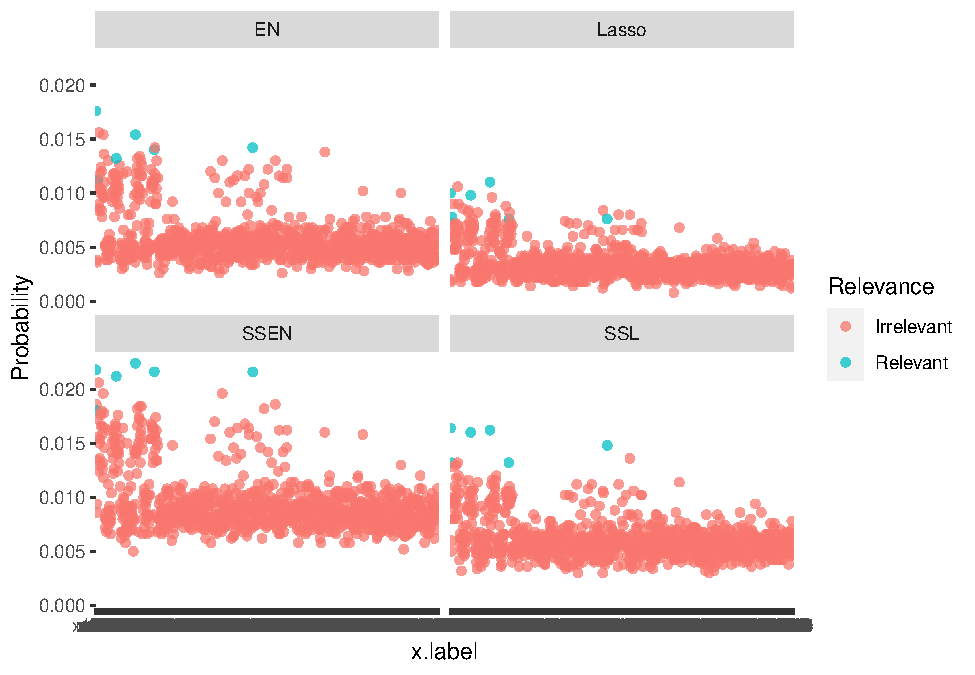
\includegraphics{simulation_results_files/figure-latex/unnamed-chunk-10-1.pdf}

\begin{longtable}[]{@{}lrrrrrr@{}}
\caption{Mean Probability of Inclusion for True Non-zero
Paramters}\tabularnewline
\toprule
Model & X1 & X51 & X101 & X151 & X201 & X251 \\
\midrule
\endfirsthead
\toprule
Model & X1 & X51 & X101 & X151 & X201 & X251 \\
\midrule
\endhead
Lasso & 0.0100 & 0.0076 & 0.0078 & 0.0098 & 0.0110 & 0.0076 \\
EN & 0.0176 & 0.0142 & 0.0112 & 0.0132 & 0.0154 & 0.0140 \\
SSL & 0.0164 & 0.0148 & 0.0132 & 0.0160 & 0.0162 & 0.0132 \\
SSEN & 0.0218 & 0.0216 & 0.0180 & 0.0212 & 0.0224 & 0.0216 \\
\bottomrule
\end{longtable}

\begin{longtable}[]{@{}llrr@{}}
\caption{Probability of Inclusion for Relevant/Irrelevant Parameters:
X1k\_B6\_BV0075015}\tabularnewline
\toprule
Model & Relevance & Mean & SD \\
\midrule
\endfirsthead
\toprule
Model & Relevance & Mean & SD \\
\midrule
\endhead
Lasso & Irrelevant & 0.0034 & 0.0014 \\
EN & Irrelevant & 0.0057 & 0.0021 \\
SSL & Irrelevant & 0.0061 & 0.0017 \\
SSEN & Irrelevant & 0.0094 & 0.0025 \\
Lasso & Relevant & 0.0090 & 0.0015 \\
EN & Relevant & 0.0143 & 0.0021 \\
SSL & Relevant & 0.0150 & 0.0015 \\
SSEN & Relevant & 0.0211 & 0.0016 \\
\bottomrule
\end{longtable}

\hypertarget{b6_bv0075015-summary-reduced-for-manuscript}{%
\subsection{B6\_BV0075015 Summary (Reduced for
Manuscript)}\label{b6_bv0075015-summary-reduced-for-manuscript}}

\begin{longtable}[]{@{}lrrrrr@{}}
\caption{Mean Model Fitness: X1k\_B6\_BV0075015}\tabularnewline
\toprule
model & s0 & s1 & deviance & FDP & Power \\
\midrule
\endfirsthead
\toprule
model & s0 & s1 & deviance & FDP & Power \\
\midrule
\endhead
Lasso & 0.1031 & 0.1031 & 216.8022 & 0.6437 & 0.0090 \\
EN & 0.2020 & 0.2020 & 216.7978 & 0.5637 & 0.0143 \\
SSL & 0.0243 & 1.7258 & 217.2746 & 0.4052 & 0.0150 \\
SSEN & 0.0152 & 1.6154 & 217.2341 & 0.3661 & 0.0211 \\
\bottomrule
\end{longtable}

\begin{longtable}[]{@{}lrrrrrr@{}}
\caption{Mean Probability of Inclusion for True Non-zero
Paramters}\tabularnewline
\toprule
Model & X1 & X51 & X101 & X151 & X201 & X251 \\
\midrule
\endfirsthead
\toprule
Model & X1 & X51 & X101 & X151 & X201 & X251 \\
\midrule
\endhead
Lasso & 0.0100 & 0.0076 & 0.0078 & 0.0098 & 0.0110 & 0.0076 \\
EN & 0.0176 & 0.0142 & 0.0112 & 0.0132 & 0.0154 & 0.0140 \\
SSL & 0.0164 & 0.0148 & 0.0132 & 0.0160 & 0.0162 & 0.0132 \\
SSEN & 0.0218 & 0.0216 & 0.0180 & 0.0212 & 0.0224 & 0.0216 \\
\bottomrule
\end{longtable}

\hypertarget{b6_b012025-summary}{%
\subsection{B6\_B012025 Summary}\label{b6_b012025-summary}}

\begin{longtable}[]{@{}
  >{\raggedright\arraybackslash}p{(\columnwidth - 22\tabcolsep) * \real{0.06}}
  >{\raggedleft\arraybackslash}p{(\columnwidth - 22\tabcolsep) * \real{0.07}}
  >{\raggedleft\arraybackslash}p{(\columnwidth - 22\tabcolsep) * \real{0.07}}
  >{\raggedleft\arraybackslash}p{(\columnwidth - 22\tabcolsep) * \real{0.09}}
  >{\raggedleft\arraybackslash}p{(\columnwidth - 22\tabcolsep) * \real{0.08}}
  >{\raggedleft\arraybackslash}p{(\columnwidth - 22\tabcolsep) * \real{0.07}}
  >{\raggedleft\arraybackslash}p{(\columnwidth - 22\tabcolsep) * \real{0.10}}
  >{\raggedleft\arraybackslash}p{(\columnwidth - 22\tabcolsep) * \real{0.09}}
  >{\raggedleft\arraybackslash}p{(\columnwidth - 22\tabcolsep) * \real{0.09}}
  >{\raggedleft\arraybackslash}p{(\columnwidth - 22\tabcolsep) * \real{0.10}}
  >{\raggedleft\arraybackslash}p{(\columnwidth - 22\tabcolsep) * \real{0.09}}
  >{\raggedleft\arraybackslash}p{(\columnwidth - 22\tabcolsep) * \real{0.09}}@{}}
\caption{Mean Model Fitness: X1k\_B6\_BV012025}\tabularnewline
\toprule
model & s0 & s1 & deviance & avg\_acc & pce & ppv\_macro & sn\_macro &
f1\_macro & ppv\_micro & sn\_micro & f1\_micro \\
\midrule
\endfirsthead
\toprule
model & s0 & s1 & deviance & avg\_acc & pce & ppv\_macro & sn\_macro &
f1\_macro & ppv\_micro & sn\_micro & f1\_micro \\
\midrule
\endhead
Lasso & 0.1001 & 0.1001 & 216.7096 & 0.5998 & 0.4002 & 0.3635 & 0.3381 &
0.3500 & 0.3996 & 0.3996 & 0.3996 \\
EN & 0.1937 & 0.1937 & 216.6557 & 0.6000 & 0.4000 & 0.3621 & 0.3386 &
0.3501 & 0.4000 & 0.4000 & 0.4000 \\
SSL & 0.0308 & 2.0642 & 217.2401 & 0.5987 & 0.4013 & 0.3636 & 0.3406 &
0.3533 & 0.3981 & 0.3981 & 0.3981 \\
SSEN & 0.0180 & 1.9542 & 217.1768 & 0.5992 & 0.4008 & 0.3673 & 0.3406 &
0.3563 & 0.3987 & 0.3987 & 0.3987 \\
\bottomrule
\end{longtable}

\begin{longtable}[]{@{}
  >{\raggedright\arraybackslash}p{(\columnwidth - 22\tabcolsep) * \real{0.06}}
  >{\raggedleft\arraybackslash}p{(\columnwidth - 22\tabcolsep) * \real{0.07}}
  >{\raggedleft\arraybackslash}p{(\columnwidth - 22\tabcolsep) * \real{0.07}}
  >{\raggedleft\arraybackslash}p{(\columnwidth - 22\tabcolsep) * \real{0.09}}
  >{\raggedleft\arraybackslash}p{(\columnwidth - 22\tabcolsep) * \real{0.08}}
  >{\raggedleft\arraybackslash}p{(\columnwidth - 22\tabcolsep) * \real{0.07}}
  >{\raggedleft\arraybackslash}p{(\columnwidth - 22\tabcolsep) * \real{0.10}}
  >{\raggedleft\arraybackslash}p{(\columnwidth - 22\tabcolsep) * \real{0.09}}
  >{\raggedleft\arraybackslash}p{(\columnwidth - 22\tabcolsep) * \real{0.09}}
  >{\raggedleft\arraybackslash}p{(\columnwidth - 22\tabcolsep) * \real{0.10}}
  >{\raggedleft\arraybackslash}p{(\columnwidth - 22\tabcolsep) * \real{0.09}}
  >{\raggedleft\arraybackslash}p{(\columnwidth - 22\tabcolsep) * \real{0.09}}@{}}
\caption{SD Model Fitness: X1k\_B6\_BV012025}\tabularnewline
\toprule
model & s0 & s1 & deviance & avg\_acc & pce & ppv\_macro & sn\_macro &
f1\_macro & ppv\_micro & sn\_micro & f1\_micro \\
\midrule
\endfirsthead
\toprule
model & s0 & s1 & deviance & avg\_acc & pce & ppv\_macro & sn\_macro &
f1\_macro & ppv\_micro & sn\_micro & f1\_micro \\
\midrule
\endhead
Lasso & 0.0172 & 0.0172 & 4.6489 & 0.0341 & 0.0341 & 0.1135 & 0.0227 &
0.0665 & 0.0511 & 0.0511 & 0.0511 \\
EN & 0.0368 & 0.0368 & 4.6383 & 0.0341 & 0.0341 & 0.1122 & 0.0236 &
0.0674 & 0.0512 & 0.0512 & 0.0512 \\
SSL & 0.0198 & 1.4328 & 5.3637 & 0.0341 & 0.0341 & 0.0989 & 0.0278 &
0.0620 & 0.0512 & 0.0512 & 0.0512 \\
SSEN & 0.0086 & 1.3963 & 5.2928 & 0.0341 & 0.0341 & 0.0958 & 0.0271 &
0.0606 & 0.0511 & 0.0511 & 0.0511 \\
\bottomrule
\end{longtable}

\begin{longtable}[]{@{}
  >{\raggedright\arraybackslash}p{(\columnwidth - 22\tabcolsep) * \real{0.06}}
  >{\raggedleft\arraybackslash}p{(\columnwidth - 22\tabcolsep) * \real{0.07}}
  >{\raggedleft\arraybackslash}p{(\columnwidth - 22\tabcolsep) * \real{0.07}}
  >{\raggedleft\arraybackslash}p{(\columnwidth - 22\tabcolsep) * \real{0.09}}
  >{\raggedleft\arraybackslash}p{(\columnwidth - 22\tabcolsep) * \real{0.08}}
  >{\raggedleft\arraybackslash}p{(\columnwidth - 22\tabcolsep) * \real{0.04}}
  >{\raggedleft\arraybackslash}p{(\columnwidth - 22\tabcolsep) * \real{0.10}}
  >{\raggedleft\arraybackslash}p{(\columnwidth - 22\tabcolsep) * \real{0.09}}
  >{\raggedleft\arraybackslash}p{(\columnwidth - 22\tabcolsep) * \real{0.09}}
  >{\raggedleft\arraybackslash}p{(\columnwidth - 22\tabcolsep) * \real{0.10}}
  >{\raggedleft\arraybackslash}p{(\columnwidth - 22\tabcolsep) * \real{0.09}}
  >{\raggedleft\arraybackslash}p{(\columnwidth - 22\tabcolsep) * \real{0.09}}@{}}
\caption{Median Model Fitness: X1k\_B6\_BV012025}\tabularnewline
\toprule
model & s0 & s1 & deviance & avg\_acc & pce & ppv\_macro & sn\_macro &
f1\_macro & ppv\_micro & sn\_micro & f1\_micro \\
\midrule
\endfirsthead
\toprule
model & s0 & s1 & deviance & avg\_acc & pce & ppv\_macro & sn\_macro &
f1\_macro & ppv\_micro & sn\_micro & f1\_micro \\
\midrule
\endhead
Lasso & 0.1029 & 0.1029 & 216.6698 & 0.6 & 0.4 & 0.3510 & 0.3333 &
0.3471 & 0.4 & 0.4 & 0.4 \\
EN & 0.1994 & 0.1994 & 216.6339 & 0.6 & 0.4 & 0.3487 & 0.3333 & 0.3483 &
0.4 & 0.4 & 0.4 \\
SSL & 0.0400 & 1.0000 & 216.9986 & 0.6 & 0.4 & 0.3527 & 0.3333 & 0.3500
& 0.4 & 0.4 & 0.4 \\
SSEN & 0.0200 & 1.0000 & 216.9323 & 0.6 & 0.4 & 0.3593 & 0.3333 & 0.3552
& 0.4 & 0.4 & 0.4 \\
\bottomrule
\end{longtable}

\begin{longtable}[]{@{}
  >{\raggedright\arraybackslash}p{(\columnwidth - 22\tabcolsep) * \real{0.06}}
  >{\raggedleft\arraybackslash}p{(\columnwidth - 22\tabcolsep) * \real{0.07}}
  >{\raggedleft\arraybackslash}p{(\columnwidth - 22\tabcolsep) * \real{0.07}}
  >{\raggedleft\arraybackslash}p{(\columnwidth - 22\tabcolsep) * \real{0.09}}
  >{\raggedleft\arraybackslash}p{(\columnwidth - 22\tabcolsep) * \real{0.08}}
  >{\raggedleft\arraybackslash}p{(\columnwidth - 22\tabcolsep) * \real{0.07}}
  >{\raggedleft\arraybackslash}p{(\columnwidth - 22\tabcolsep) * \real{0.10}}
  >{\raggedleft\arraybackslash}p{(\columnwidth - 22\tabcolsep) * \real{0.09}}
  >{\raggedleft\arraybackslash}p{(\columnwidth - 22\tabcolsep) * \real{0.09}}
  >{\raggedleft\arraybackslash}p{(\columnwidth - 22\tabcolsep) * \real{0.10}}
  >{\raggedleft\arraybackslash}p{(\columnwidth - 22\tabcolsep) * \real{0.09}}
  >{\raggedleft\arraybackslash}p{(\columnwidth - 22\tabcolsep) * \real{0.09}}@{}}
\caption{IQR Model Fitness: X1k\_B6\_BV012025}\tabularnewline
\toprule
model & s0 & s1 & deviance & avg\_acc & pce & ppv\_macro & sn\_macro &
f1\_macro & ppv\_micro & sn\_micro & f1\_micro \\
\midrule
\endfirsthead
\toprule
model & s0 & s1 & deviance & avg\_acc & pce & ppv\_macro & sn\_macro &
f1\_macro & ppv\_micro & sn\_micro & f1\_micro \\
\midrule
\endhead
Lasso & 0.0254 & 0.0254 & 5.5223 & 0.0417 & 0.0417 & 0.1449 & 0.0050 &
0.0932 & 0.0625 & 0.0625 & 0.0625 \\
EN & 0.0579 & 0.0579 & 5.5248 & 0.0400 & 0.0400 & 0.1497 & 0.0074 &
0.0992 & 0.0600 & 0.0600 & 0.0600 \\
SSL & 0.0400 & 3.0000 & 6.2586 & 0.0467 & 0.0467 & 0.1229 & 0.0126 &
0.0865 & 0.0700 & 0.0700 & 0.0700 \\
SSEN & 0.0200 & 3.0000 & 6.1332 & 0.0467 & 0.0467 & 0.1168 & 0.0120 &
0.0858 & 0.0700 & 0.0700 & 0.0700 \\
\bottomrule
\end{longtable}

\begin{longtable}[]{@{}lrrr@{}}
\caption{Mean False Positive Rates and Power:
X1k\_B6\_BV012025}\tabularnewline
\toprule
model & FDP & FWE & Power \\
\midrule
\endfirsthead
\toprule
model & FDP & FWE & Power \\
\midrule
\endhead
Lasso & 0.7166 & 0.7396 & 0.0338 \\
EN & 0.6555 & 0.6802 & 0.0557 \\
SSL & 0.5435 & 0.5608 & 0.0479 \\
SSEN & 0.5100 & 0.5262 & 0.0697 \\
\bottomrule
\end{longtable}

\begin{longtable}[]{@{}lrrr@{}}
\caption{SD False Positive Rates and Power:
X1k\_B6\_BV012025}\tabularnewline
\toprule
model & FDP & FWE & Power \\
\midrule
\endfirsthead
\toprule
model & FDP & FWE & Power \\
\midrule
\endhead
Lasso & 0.4308 & 0.4389 & 0.0789 \\
EN & 0.4536 & 0.4664 & 0.1038 \\
SSL & 0.4828 & 0.4963 & 0.0984 \\
SSEN & 0.4849 & 0.4994 & 0.1235 \\
\bottomrule
\end{longtable}

\begin{longtable}[]{@{}lrrr@{}}
\caption{Median False Positive Rates and Power:
X1k\_B6\_BV012025}\tabularnewline
\toprule
model & FDP & FWE & Power \\
\midrule
\endfirsthead
\toprule
model & FDP & FWE & Power \\
\midrule
\endhead
Lasso & 1.0000 & 1 & 0 \\
EN & 0.9565 & 1 & 0 \\
SSL & 0.9000 & 1 & 0 \\
SSEN & 0.8889 & 1 & 0 \\
\bottomrule
\end{longtable}

\begin{longtable}[]{@{}lrrr@{}}
\caption{IQR False Positive Rates and Power:
X1k\_B6\_BV012025}\tabularnewline
\toprule
model & FDP & FWE & Power \\
\midrule
\endfirsthead
\toprule
model & FDP & FWE & Power \\
\midrule
\endhead
Lasso & 1.0000 & 1 & 0.0000 \\
EN & 1.0000 & 1 & 0.1667 \\
SSL & 1.0000 & 1 & 0.0000 \\
SSEN & 0.9828 & 1 & 0.1667 \\
\bottomrule
\end{longtable}

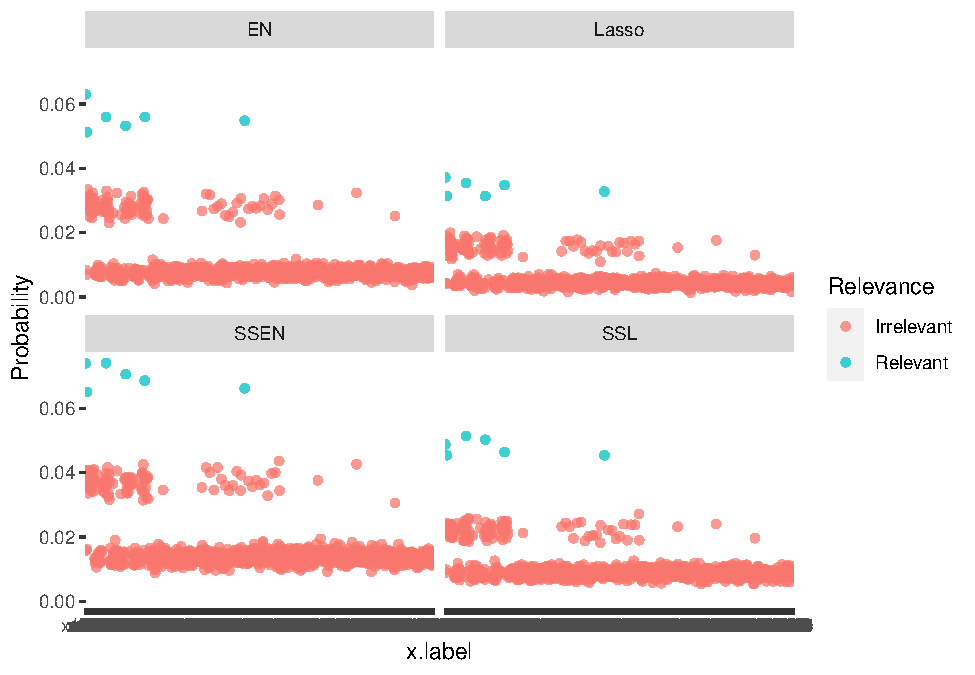
\includegraphics{simulation_results_files/figure-latex/unnamed-chunk-13-1.pdf}

\begin{longtable}[]{@{}lrrrrrr@{}}
\caption{Mean Probability of Inclusion for True Non-zero
Paramters}\tabularnewline
\toprule
Model & X1 & X51 & X101 & X151 & X201 & X251 \\
\midrule
\endfirsthead
\toprule
Model & X1 & X51 & X101 & X151 & X201 & X251 \\
\midrule
\endhead
Lasso & 0.0372 & 0.0328 & 0.0314 & 0.0354 & 0.0314 & 0.0348 \\
EN & 0.0630 & 0.0548 & 0.0512 & 0.0560 & 0.0532 & 0.0560 \\
SSL & 0.0488 & 0.0454 & 0.0454 & 0.0514 & 0.0502 & 0.0464 \\
SSEN & 0.0740 & 0.0662 & 0.0650 & 0.0740 & 0.0706 & 0.0686 \\
\bottomrule
\end{longtable}

\begin{longtable}[]{@{}llrr@{}}
\caption{Probability of Inclusion for Relevant/Irrelevant Parameters:
X1k\_B6\_BV012025}\tabularnewline
\toprule
Model & Relevance & Mean & SD \\
\midrule
\endfirsthead
\toprule
Model & Relevance & Mean & SD \\
\midrule
\endhead
Lasso & Irrelevant & 0.0056 & 0.0038 \\
EN & Irrelevant & 0.0099 & 0.0067 \\
SSL & Irrelevant & 0.0103 & 0.0044 \\
SSEN & Irrelevant & 0.0163 & 0.0076 \\
Lasso & Relevant & 0.0338 & 0.0024 \\
EN & Relevant & 0.0557 & 0.0040 \\
SSL & Relevant & 0.0479 & 0.0026 \\
SSEN & Relevant & 0.0697 & 0.0038 \\
\bottomrule
\end{longtable}

\hypertarget{b6_bv012025-summary-reduced-for-manuscript}{%
\subsection{B6\_BV012025 Summary (Reduced for
Manuscript)}\label{b6_bv012025-summary-reduced-for-manuscript}}

\begin{longtable}[]{@{}lrrrrr@{}}
\caption{Mean Model Fitness: X1k\_B6\_BV012025}\tabularnewline
\toprule
model & s0 & s1 & deviance & FDP & Power \\
\midrule
\endfirsthead
\toprule
model & s0 & s1 & deviance & FDP & Power \\
\midrule
\endhead
Lasso & 0.1001 & 0.1001 & 216.7096 & 0.7166 & 0.0338 \\
EN & 0.1937 & 0.1937 & 216.6557 & 0.6555 & 0.0557 \\
SSL & 0.0308 & 2.0642 & 217.2401 & 0.5435 & 0.0479 \\
SSEN & 0.0180 & 1.9542 & 217.1768 & 0.5100 & 0.0697 \\
\bottomrule
\end{longtable}

\begin{longtable}[]{@{}lrrrrrr@{}}
\caption{Mean Probability of Inclusion for True Non-zero
Paramters}\tabularnewline
\toprule
Model & X1 & X51 & X101 & X151 & X201 & X251 \\
\midrule
\endfirsthead
\toprule
Model & X1 & X51 & X101 & X151 & X201 & X251 \\
\midrule
\endhead
Lasso & 0.0372 & 0.0328 & 0.0314 & 0.0354 & 0.0314 & 0.0348 \\
EN & 0.0630 & 0.0548 & 0.0512 & 0.0560 & 0.0532 & 0.0560 \\
SSL & 0.0488 & 0.0454 & 0.0454 & 0.0514 & 0.0502 & 0.0464 \\
SSEN & 0.0740 & 0.0662 & 0.0650 & 0.0740 & 0.0706 & 0.0686 \\
\bottomrule
\end{longtable}

\hypertarget{b6_b025050-summary}{%
\subsection{B6\_B025050 Summary}\label{b6_b025050-summary}}

\begin{longtable}[]{@{}
  >{\raggedright\arraybackslash}p{(\columnwidth - 22\tabcolsep) * \real{0.06}}
  >{\raggedleft\arraybackslash}p{(\columnwidth - 22\tabcolsep) * \real{0.07}}
  >{\raggedleft\arraybackslash}p{(\columnwidth - 22\tabcolsep) * \real{0.07}}
  >{\raggedleft\arraybackslash}p{(\columnwidth - 22\tabcolsep) * \real{0.09}}
  >{\raggedleft\arraybackslash}p{(\columnwidth - 22\tabcolsep) * \real{0.08}}
  >{\raggedleft\arraybackslash}p{(\columnwidth - 22\tabcolsep) * \real{0.07}}
  >{\raggedleft\arraybackslash}p{(\columnwidth - 22\tabcolsep) * \real{0.10}}
  >{\raggedleft\arraybackslash}p{(\columnwidth - 22\tabcolsep) * \real{0.09}}
  >{\raggedleft\arraybackslash}p{(\columnwidth - 22\tabcolsep) * \real{0.09}}
  >{\raggedleft\arraybackslash}p{(\columnwidth - 22\tabcolsep) * \real{0.10}}
  >{\raggedleft\arraybackslash}p{(\columnwidth - 22\tabcolsep) * \real{0.09}}
  >{\raggedleft\arraybackslash}p{(\columnwidth - 22\tabcolsep) * \real{0.09}}@{}}
\caption{Mean Model Fitness: X1k\_B6\_BV025050}\tabularnewline
\toprule
model & s0 & s1 & deviance & avg\_acc & pce & ppv\_macro & sn\_macro &
f1\_macro & ppv\_micro & sn\_micro & f1\_micro \\
\midrule
\endfirsthead
\toprule
model & s0 & s1 & deviance & avg\_acc & pce & ppv\_macro & sn\_macro &
f1\_macro & ppv\_micro & sn\_micro & f1\_micro \\
\midrule
\endhead
Lasso & 0.0770 & 0.0770 & 210.9040 & 0.6259 & 0.3741 & 0.4224 & 0.3923 &
0.4081 & 0.4389 & 0.4389 & 0.4389 \\
EN & 0.1445 & 0.1445 & 210.6891 & 0.6268 & 0.3732 & 0.4243 & 0.3935 &
0.4094 & 0.4402 & 0.4402 & 0.4402 \\
SSL & 0.0553 & 3.0590 & 210.9524 & 0.6275 & 0.3725 & 0.4210 & 0.4030 &
0.4129 & 0.4412 & 0.4412 & 0.4412 \\
SSEN & 0.0301 & 2.9224 & 210.8284 & 0.6278 & 0.3722 & 0.4231 & 0.4036 &
0.4145 & 0.4417 & 0.4417 & 0.4417 \\
\bottomrule
\end{longtable}

\begin{longtable}[]{@{}
  >{\raggedright\arraybackslash}p{(\columnwidth - 22\tabcolsep) * \real{0.06}}
  >{\raggedleft\arraybackslash}p{(\columnwidth - 22\tabcolsep) * \real{0.07}}
  >{\raggedleft\arraybackslash}p{(\columnwidth - 22\tabcolsep) * \real{0.07}}
  >{\raggedleft\arraybackslash}p{(\columnwidth - 22\tabcolsep) * \real{0.09}}
  >{\raggedleft\arraybackslash}p{(\columnwidth - 22\tabcolsep) * \real{0.08}}
  >{\raggedleft\arraybackslash}p{(\columnwidth - 22\tabcolsep) * \real{0.07}}
  >{\raggedleft\arraybackslash}p{(\columnwidth - 22\tabcolsep) * \real{0.10}}
  >{\raggedleft\arraybackslash}p{(\columnwidth - 22\tabcolsep) * \real{0.09}}
  >{\raggedleft\arraybackslash}p{(\columnwidth - 22\tabcolsep) * \real{0.09}}
  >{\raggedleft\arraybackslash}p{(\columnwidth - 22\tabcolsep) * \real{0.10}}
  >{\raggedleft\arraybackslash}p{(\columnwidth - 22\tabcolsep) * \real{0.09}}
  >{\raggedleft\arraybackslash}p{(\columnwidth - 22\tabcolsep) * \real{0.09}}@{}}
\caption{SD Model Fitness: X1k\_B6\_BV025050}\tabularnewline
\toprule
model & s0 & s1 & deviance & avg\_acc & pce & ppv\_macro & sn\_macro &
f1\_macro & ppv\_micro & sn\_micro & f1\_micro \\
\midrule
\endfirsthead
\toprule
model & s0 & s1 & deviance & avg\_acc & pce & ppv\_macro & sn\_macro &
f1\_macro & ppv\_micro & sn\_micro & f1\_micro \\
\midrule
\endhead
Lasso & 0.0149 & 0.0149 & 6.5346 & 0.0351 & 0.0351 & 0.0876 & 0.0470 &
0.0591 & 0.0526 & 0.0526 & 0.0526 \\
EN & 0.0290 & 0.0290 & 6.4617 & 0.0348 & 0.0348 & 0.0882 & 0.0469 &
0.0593 & 0.0521 & 0.0521 & 0.0521 \\
SSL & 0.0132 & 1.3769 & 7.7893 & 0.0348 & 0.0348 & 0.0716 & 0.0489 &
0.0550 & 0.0522 & 0.0522 & 0.0522 \\
SSEN & 0.0067 & 1.4355 & 7.7913 & 0.0352 & 0.0352 & 0.0720 & 0.0490 &
0.0552 & 0.0527 & 0.0527 & 0.0527 \\
\bottomrule
\end{longtable}

\begin{longtable}[]{@{}
  >{\raggedright\arraybackslash}p{(\columnwidth - 22\tabcolsep) * \real{0.06}}
  >{\raggedleft\arraybackslash}p{(\columnwidth - 22\tabcolsep) * \real{0.07}}
  >{\raggedleft\arraybackslash}p{(\columnwidth - 22\tabcolsep) * \real{0.07}}
  >{\raggedleft\arraybackslash}p{(\columnwidth - 22\tabcolsep) * \real{0.09}}
  >{\raggedleft\arraybackslash}p{(\columnwidth - 22\tabcolsep) * \real{0.08}}
  >{\raggedleft\arraybackslash}p{(\columnwidth - 22\tabcolsep) * \real{0.07}}
  >{\raggedleft\arraybackslash}p{(\columnwidth - 22\tabcolsep) * \real{0.10}}
  >{\raggedleft\arraybackslash}p{(\columnwidth - 22\tabcolsep) * \real{0.09}}
  >{\raggedleft\arraybackslash}p{(\columnwidth - 22\tabcolsep) * \real{0.09}}
  >{\raggedleft\arraybackslash}p{(\columnwidth - 22\tabcolsep) * \real{0.10}}
  >{\raggedleft\arraybackslash}p{(\columnwidth - 22\tabcolsep) * \real{0.09}}
  >{\raggedleft\arraybackslash}p{(\columnwidth - 22\tabcolsep) * \real{0.09}}@{}}
\caption{Median Model Fitness: X1k\_B6\_BV025050}\tabularnewline
\toprule
model & s0 & s1 & deviance & avg\_acc & pce & ppv\_macro & sn\_macro &
f1\_macro & ppv\_micro & sn\_micro & f1\_micro \\
\midrule
\endfirsthead
\toprule
model & s0 & s1 & deviance & avg\_acc & pce & ppv\_macro & sn\_macro &
f1\_macro & ppv\_micro & sn\_micro & f1\_micro \\
\midrule
\endhead
Lasso & 0.0746 & 0.0746 & 211.1127 & 0.6267 & 0.3733 & 0.4212 & 0.3905 &
0.4091 & 0.44 & 0.44 & 0.44 \\
EN & 0.1397 & 0.1397 & 210.8755 & 0.6267 & 0.3733 & 0.4220 & 0.3914 &
0.4109 & 0.44 & 0.44 & 0.44 \\
SSL & 0.0600 & 4.0000 & 211.0422 & 0.6267 & 0.3733 & 0.4201 & 0.4019 &
0.4134 & 0.44 & 0.44 & 0.44 \\
SSEN & 0.0300 & 4.0000 & 210.9342 & 0.6267 & 0.3733 & 0.4223 & 0.4034 &
0.4155 & 0.44 & 0.44 & 0.44 \\
\bottomrule
\end{longtable}

\begin{longtable}[]{@{}
  >{\raggedright\arraybackslash}p{(\columnwidth - 22\tabcolsep) * \real{0.06}}
  >{\raggedleft\arraybackslash}p{(\columnwidth - 22\tabcolsep) * \real{0.07}}
  >{\raggedleft\arraybackslash}p{(\columnwidth - 22\tabcolsep) * \real{0.07}}
  >{\raggedleft\arraybackslash}p{(\columnwidth - 22\tabcolsep) * \real{0.09}}
  >{\raggedleft\arraybackslash}p{(\columnwidth - 22\tabcolsep) * \real{0.08}}
  >{\raggedleft\arraybackslash}p{(\columnwidth - 22\tabcolsep) * \real{0.07}}
  >{\raggedleft\arraybackslash}p{(\columnwidth - 22\tabcolsep) * \real{0.10}}
  >{\raggedleft\arraybackslash}p{(\columnwidth - 22\tabcolsep) * \real{0.09}}
  >{\raggedleft\arraybackslash}p{(\columnwidth - 22\tabcolsep) * \real{0.09}}
  >{\raggedleft\arraybackslash}p{(\columnwidth - 22\tabcolsep) * \real{0.10}}
  >{\raggedleft\arraybackslash}p{(\columnwidth - 22\tabcolsep) * \real{0.09}}
  >{\raggedleft\arraybackslash}p{(\columnwidth - 22\tabcolsep) * \real{0.09}}@{}}
\caption{IQR Model Fitness: X1k\_B6\_BV025050}\tabularnewline
\toprule
model & s0 & s1 & deviance & avg\_acc & pce & ppv\_macro & sn\_macro &
f1\_macro & ppv\_micro & sn\_micro & f1\_micro \\
\midrule
\endfirsthead
\toprule
model & s0 & s1 & deviance & avg\_acc & pce & ppv\_macro & sn\_macro &
f1\_macro & ppv\_micro & sn\_micro & f1\_micro \\
\midrule
\endhead
Lasso & 0.0167 & 0.0167 & 8.4828 & 0.0467 & 0.0467 & 0.1064 & 0.0690 &
0.0775 & 0.07 & 0.07 & 0.07 \\
EN & 0.0318 & 0.0318 & 8.4177 & 0.0467 & 0.0467 & 0.1057 & 0.0686 &
0.0787 & 0.07 & 0.07 & 0.07 \\
SSL & 0.0100 & 3.0000 & 9.9019 & 0.0467 & 0.0467 & 0.0899 & 0.0673 &
0.0726 & 0.07 & 0.07 & 0.07 \\
SSEN & 0.0000 & 3.0000 & 10.0360 & 0.0467 & 0.0467 & 0.0886 & 0.0690 &
0.0723 & 0.07 & 0.07 & 0.07 \\
\bottomrule
\end{longtable}

\begin{longtable}[]{@{}lrrr@{}}
\caption{Mean False Positive Rates and Power:
X1k\_B6\_BV025050}\tabularnewline
\toprule
model & FDP & FWE & Power \\
\midrule
\endfirsthead
\toprule
model & FDP & FWE & Power \\
\midrule
\endhead
Lasso & 0.8917 & 0.9802 & 0.2519 \\
EN & 0.9067 & 0.9808 & 0.3799 \\
SSL & 0.9016 & 0.9616 & 0.2955 \\
SSEN & 0.9139 & 0.9656 & 0.4264 \\
\bottomrule
\end{longtable}

\begin{longtable}[]{@{}lrrr@{}}
\caption{SD False Positive Rates and Power:
X1k\_B6\_BV025050}\tabularnewline
\toprule
model & FDP & FWE & Power \\
\midrule
\endfirsthead
\toprule
model & FDP & FWE & Power \\
\midrule
\endhead
Lasso & 0.1519 & 0.1393 & 0.1894 \\
EN & 0.1384 & 0.1372 & 0.2158 \\
SSL & 0.1867 & 0.1922 & 0.1977 \\
SSEN & 0.1758 & 0.1823 & 0.2211 \\
\bottomrule
\end{longtable}

\begin{longtable}[]{@{}lrrr@{}}
\caption{Median False Positive Rates and Power:
X1k\_B6\_BV025050}\tabularnewline
\toprule
model & FDP & FWE & Power \\
\midrule
\endfirsthead
\toprule
model & FDP & FWE & Power \\
\midrule
\endhead
Lasso & 0.9231 & 1 & 0.1667 \\
EN & 0.9322 & 1 & 0.3333 \\
SSL & 0.9444 & 1 & 0.3333 \\
SSEN & 0.9500 & 1 & 0.5000 \\
\bottomrule
\end{longtable}

\begin{longtable}[]{@{}lrrr@{}}
\caption{IQR False Positive Rates and Power:
X1k\_B6\_BV025050}\tabularnewline
\toprule
model & FDP & FWE & Power \\
\midrule
\endfirsthead
\toprule
model & FDP & FWE & Power \\
\midrule
\endhead
Lasso & 0.0934 & 0 & 0.1667 \\
EN & 0.0583 & 0 & 0.3333 \\
SSL & 0.0570 & 0 & 0.3333 \\
SSEN & 0.0357 & 0 & 0.1667 \\
\bottomrule
\end{longtable}

\begin{longtable}[]{@{}lrrrrrr@{}}
\caption{Mean Probability of Inclusion for True Non-zero
Paramters}\tabularnewline
\toprule
Model & X1 & X51 & X101 & X151 & X201 & X251 \\
\midrule
\endfirsthead
\toprule
Model & X1 & X51 & X101 & X151 & X201 & X251 \\
\midrule
\endhead
Lasso & 0.2514 & 0.2522 & 0.2492 & 0.2492 & 0.2504 & 0.2588 \\
EN & 0.3772 & 0.3792 & 0.3800 & 0.3770 & 0.3778 & 0.3880 \\
SSL & 0.2922 & 0.2900 & 0.2916 & 0.2964 & 0.2982 & 0.3046 \\
SSEN & 0.4196 & 0.4238 & 0.4292 & 0.4270 & 0.4286 & 0.4302 \\
\bottomrule
\end{longtable}

\begin{longtable}[]{@{}llrr@{}}
\caption{Probability of Inclusion for Relevant/Irrelevant Parameters:
X1k\_B6\_BV025050}\tabularnewline
\toprule
Model & Relevance & Mean & SD \\
\midrule
\endfirsthead
\toprule
Model & Relevance & Mean & SD \\
\midrule
\endhead
Lasso & Irrelevant & 0.0181 & 0.0174 \\
EN & Irrelevant & 0.0327 & 0.0347 \\
SSL & Irrelevant & 0.0302 & 0.0184 \\
SSEN & Irrelevant & 0.0513 & 0.0356 \\
Lasso & Relevant & 0.2519 & 0.0036 \\
EN & Relevant & 0.3799 & 0.0042 \\
SSL & Relevant & 0.2955 & 0.0054 \\
SSEN & Relevant & 0.4264 & 0.0040 \\
\bottomrule
\end{longtable}

\hypertarget{b6_bv025050-summary-reduced-for-manuscript}{%
\subsection{B6\_BV025050 Summary (Reduced for
Manuscript)}\label{b6_bv025050-summary-reduced-for-manuscript}}

\begin{longtable}[]{@{}lrrrrr@{}}
\caption{Mean Model Fitness: X1k\_B6\_BV025050}\tabularnewline
\toprule
model & s0 & s1 & deviance & FDP & Power \\
\midrule
\endfirsthead
\toprule
model & s0 & s1 & deviance & FDP & Power \\
\midrule
\endhead
Lasso & 0.0770 & 0.0770 & 210.9040 & 0.8917 & 0.2519 \\
EN & 0.1445 & 0.1445 & 210.6891 & 0.9067 & 0.3799 \\
SSL & 0.0553 & 3.0590 & 210.9524 & 0.9016 & 0.2955 \\
SSEN & 0.0301 & 2.9224 & 210.8284 & 0.9139 & 0.4264 \\
\bottomrule
\end{longtable}

\begin{longtable}[]{@{}lrrrrrr@{}}
\caption{Mean Probability of Inclusion for True Non-zero
Paramters}\tabularnewline
\toprule
Model & X1 & X51 & X101 & X151 & X201 & X251 \\
\midrule
\endfirsthead
\toprule
Model & X1 & X51 & X101 & X151 & X201 & X251 \\
\midrule
\endhead
Lasso & 0.2514 & 0.2522 & 0.2492 & 0.2492 & 0.2504 & 0.2588 \\
EN & 0.3772 & 0.3792 & 0.3800 & 0.3770 & 0.3778 & 0.3880 \\
SSL & 0.2922 & 0.2900 & 0.2916 & 0.2964 & 0.2982 & 0.3046 \\
SSEN & 0.4196 & 0.4238 & 0.4292 & 0.4270 & 0.4286 & 0.4302 \\
\bottomrule
\end{longtable}

\hypertarget{summary-reduced-for-manuscript}{%
\subsection{Summary (Reduced for
Manuscript)}\label{summary-reduced-for-manuscript}}

\begin{longtable}[]{@{}llrrrrr@{}}
\toprule
scenario & model & s0 & s1 & deviance & FDP & Power \\
\midrule
\endhead
Scenario 1 & Lasso & 0.1031141 & 0.1031141 & 216.8022 & 0.6437452 &
0.0089667 \\
Scenario 1 & EN & 0.2020326 & 0.2020326 & 216.7978 & 0.5637058 &
0.0142667 \\
Scenario 1 & SSL & 0.0242820 & 1.7258000 & 217.2746 & 0.4052290 &
0.0149667 \\
Scenario 1 & SSEN & 0.0151680 & 1.6154000 & 217.2341 & 0.3661322 &
0.0211000 \\
Scenario 2 & Lasso & 0.1000553 & 0.1000553 & 216.7096 & 0.7166263 &
0.0338333 \\
Scenario 2 & EN & 0.1936949 & 0.1936949 & 216.6557 & 0.6555374 &
0.0557000 \\
Scenario 2 & SSL & 0.0307700 & 2.0642000 & 217.2401 & 0.5434850 &
0.0479333 \\
Scenario 2 & SSEN & 0.0179940 & 1.9542000 & 217.1768 & 0.5099825 &
0.0697333 \\
Scenario 3 & Lasso & 0.0770487 & 0.0770487 & 210.9040 & 0.8917342 &
0.2518667 \\
Scenario 3 & EN & 0.1445050 & 0.1445050 & 210.6891 & 0.9066802 &
0.3798667 \\
Scenario 3 & SSL & 0.0553260 & 3.0590000 & 210.9524 & 0.9015955 &
0.2955000 \\
Scenario 3 & SSEN & 0.0301220 & 2.9224000 & 210.8284 & 0.9139263 &
0.4264000 \\
\bottomrule
\end{longtable}

\begin{longtable}[]{@{}llrrrrrr@{}}
\toprule
Scenario & Model & X1 & X51 & X101 & X151 & X201 & X251 \\
\midrule
\endhead
Scenario 1 & Lasso & 0.0100 & 0.0076 & 0.0078 & 0.0098 & 0.0110 &
0.0076 \\
Scenario 1 & EN & 0.0176 & 0.0142 & 0.0112 & 0.0132 & 0.0154 & 0.0140 \\
Scenario 1 & SSL & 0.0164 & 0.0148 & 0.0132 & 0.0160 & 0.0162 &
0.0132 \\
Scenario 1 & SSEN & 0.0218 & 0.0216 & 0.0180 & 0.0212 & 0.0224 &
0.0216 \\
Scenario 2 & Lasso & 0.0372 & 0.0328 & 0.0314 & 0.0354 & 0.0314 &
0.0348 \\
Scenario 2 & EN & 0.0630 & 0.0548 & 0.0512 & 0.0560 & 0.0532 & 0.0560 \\
Scenario 2 & SSL & 0.0488 & 0.0454 & 0.0454 & 0.0514 & 0.0502 &
0.0464 \\
Scenario 2 & SSEN & 0.0740 & 0.0662 & 0.0650 & 0.0740 & 0.0706 &
0.0686 \\
Scenario 3 & Lasso & 0.2514 & 0.2522 & 0.2492 & 0.2492 & 0.2504 &
0.2588 \\
Scenario 3 & EN & 0.3772 & 0.3792 & 0.3800 & 0.3770 & 0.3778 & 0.3880 \\
Scenario 3 & SSL & 0.2922 & 0.2900 & 0.2916 & 0.2964 & 0.2982 &
0.3046 \\
Scenario 3 & SSEN & 0.4196 & 0.4238 & 0.4292 & 0.4270 & 0.4286 &
0.4302 \\
\bottomrule
\end{longtable}

\hypertarget{plots}{%
\section{Plots}\label{plots}}

\hypertarget{inclusion-probabilities}{%
\subsection{Inclusion Probabilities}\label{inclusion-probabilities}}

\begin{verbatim}
## Warning: Using alpha for a discrete variable is not advised.
\end{verbatim}

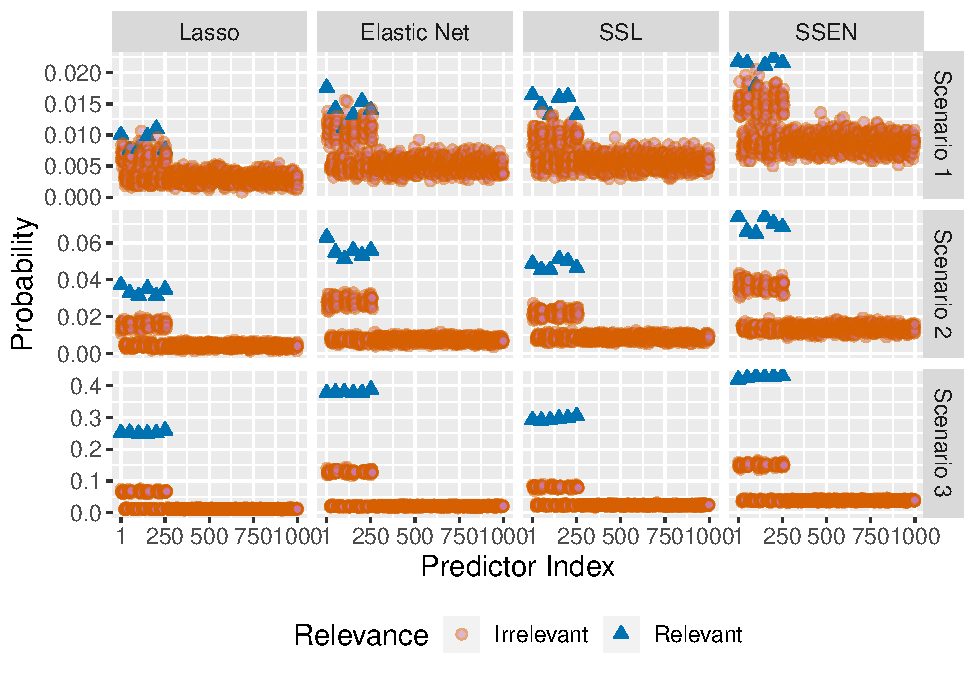
\includegraphics{simulation_results_files/figure-latex/unnamed-chunk-20-1.pdf}
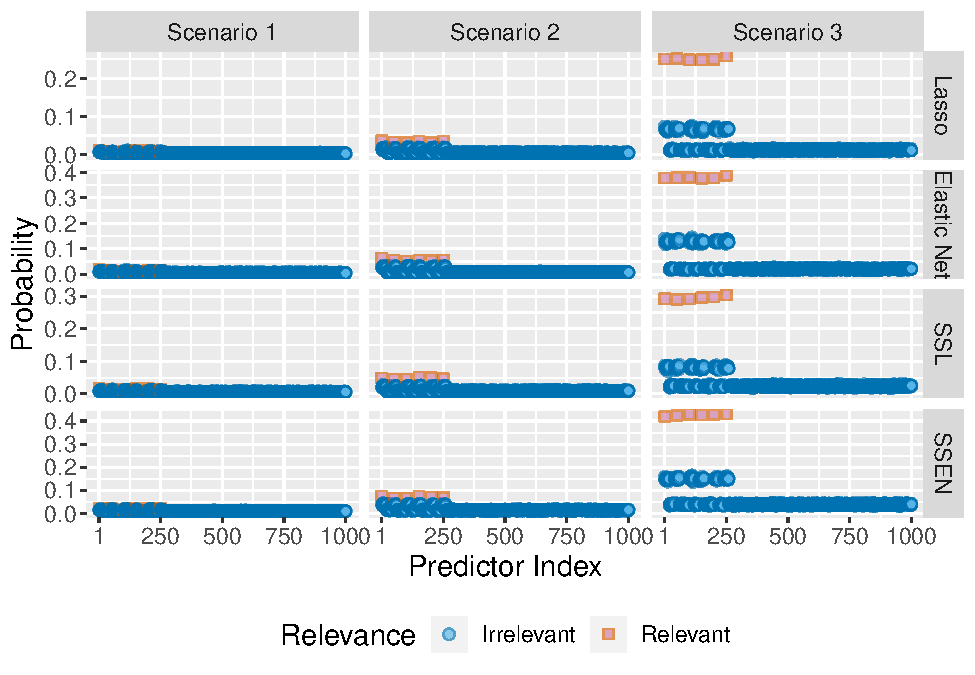
\includegraphics{simulation_results_files/figure-latex/unnamed-chunk-20-2.pdf}
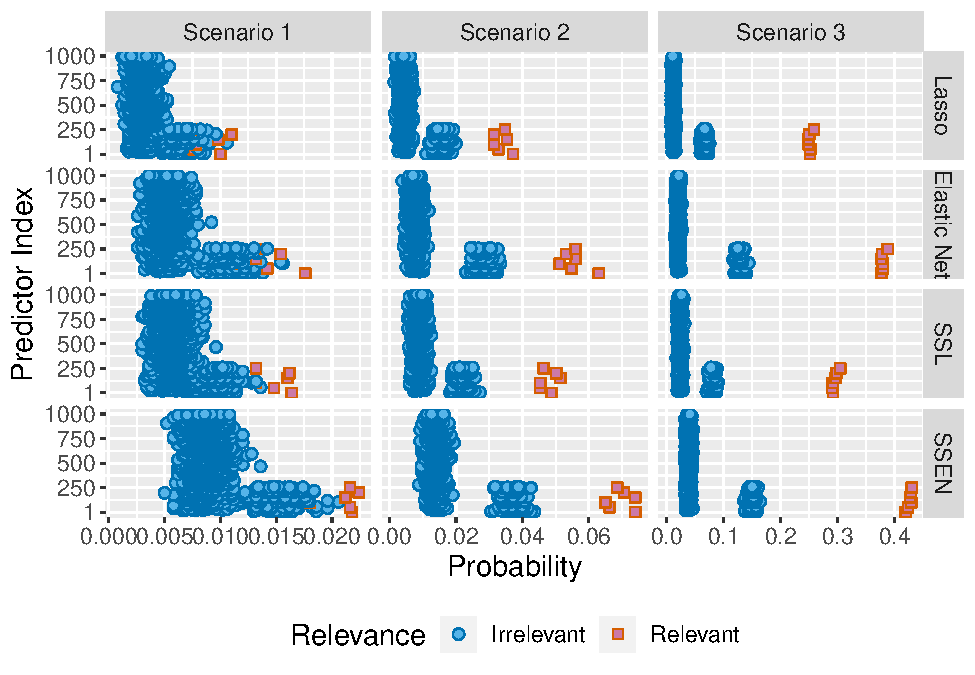
\includegraphics{simulation_results_files/figure-latex/unnamed-chunk-20-3.pdf}

\hypertarget{fdp}{%
\subsection{FDP}\label{fdp}}

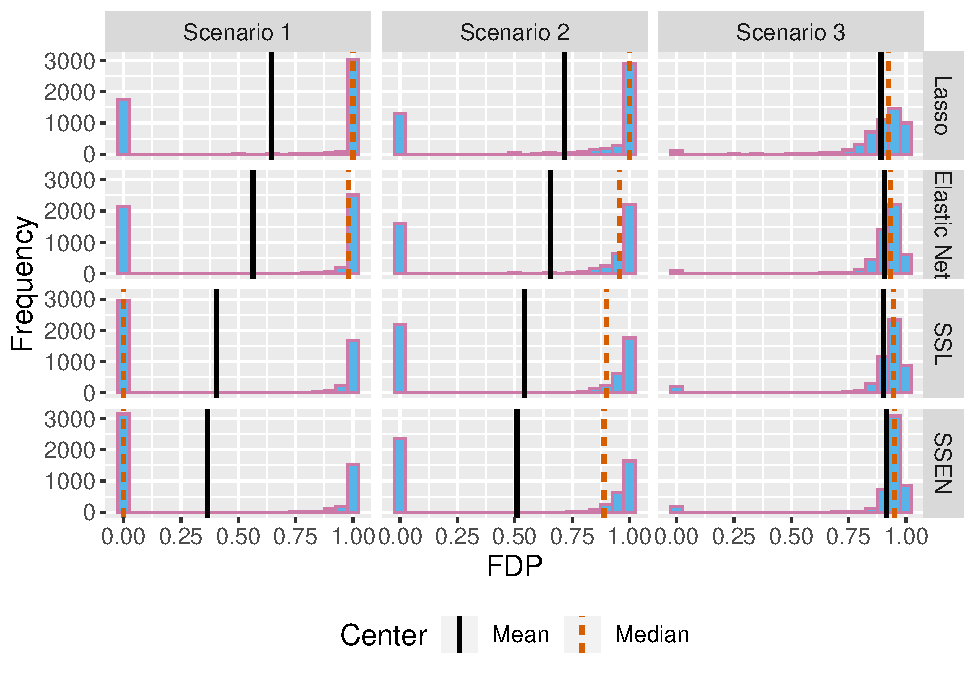
\includegraphics{simulation_results_files/figure-latex/unnamed-chunk-22-1.pdf}
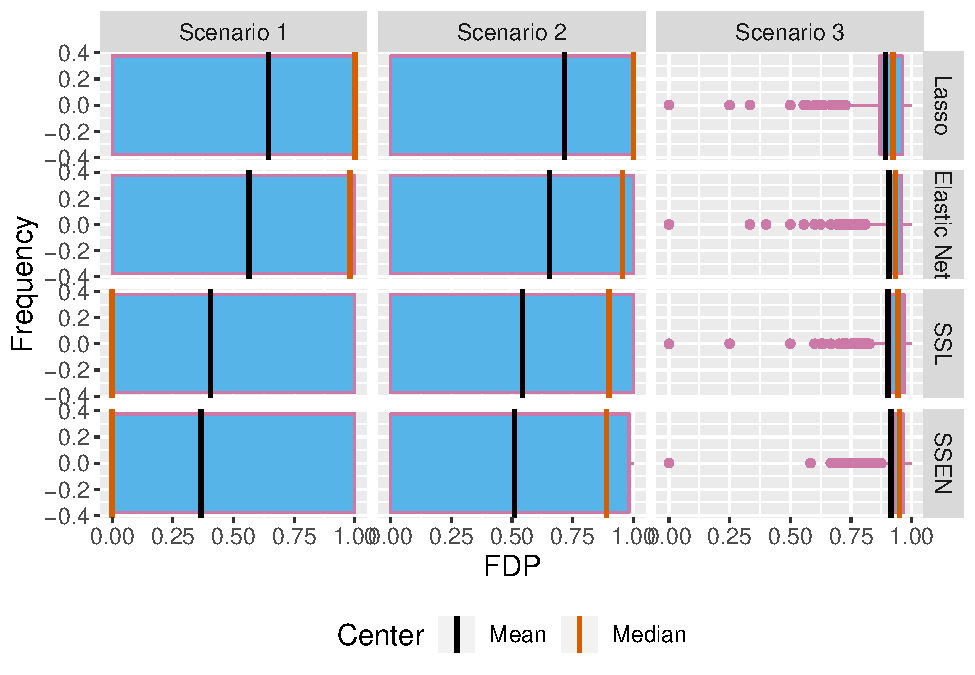
\includegraphics{simulation_results_files/figure-latex/unnamed-chunk-22-2.pdf}

\hypertarget{fwe}{%
\subsection{FWE}\label{fwe}}

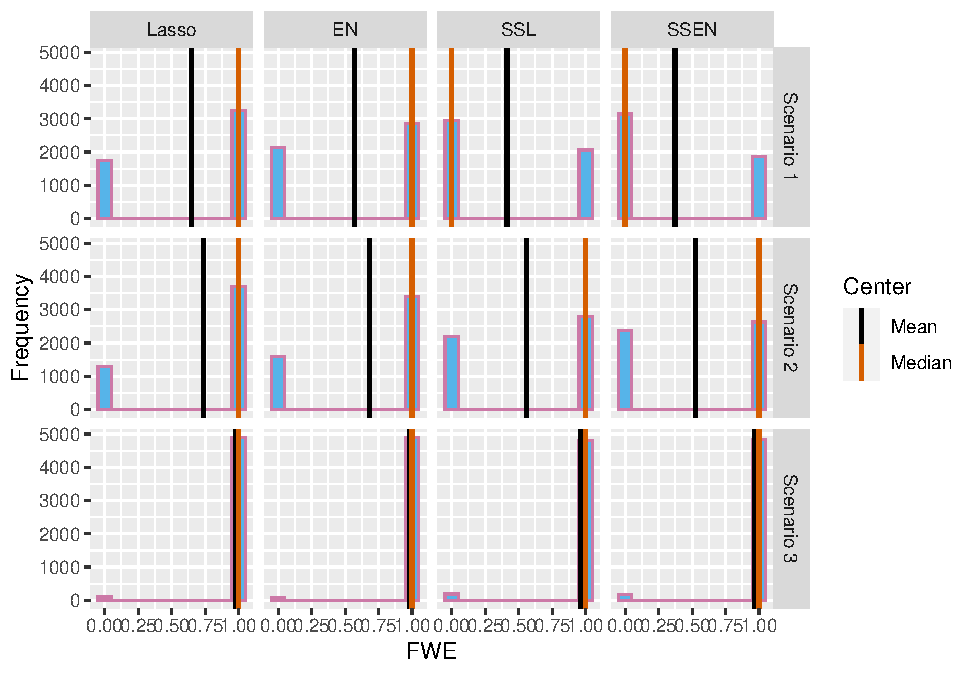
\includegraphics{simulation_results_files/figure-latex/unnamed-chunk-23-1.pdf}

\hypertarget{power}{%
\subsection{Power}\label{power}}

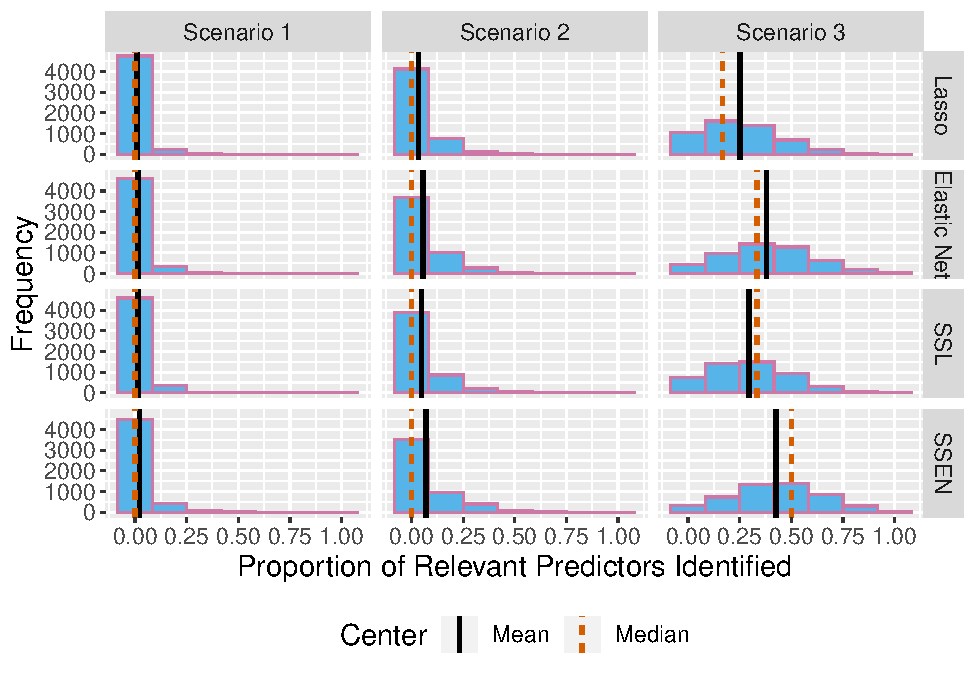
\includegraphics{simulation_results_files/figure-latex/unnamed-chunk-24-1.pdf}
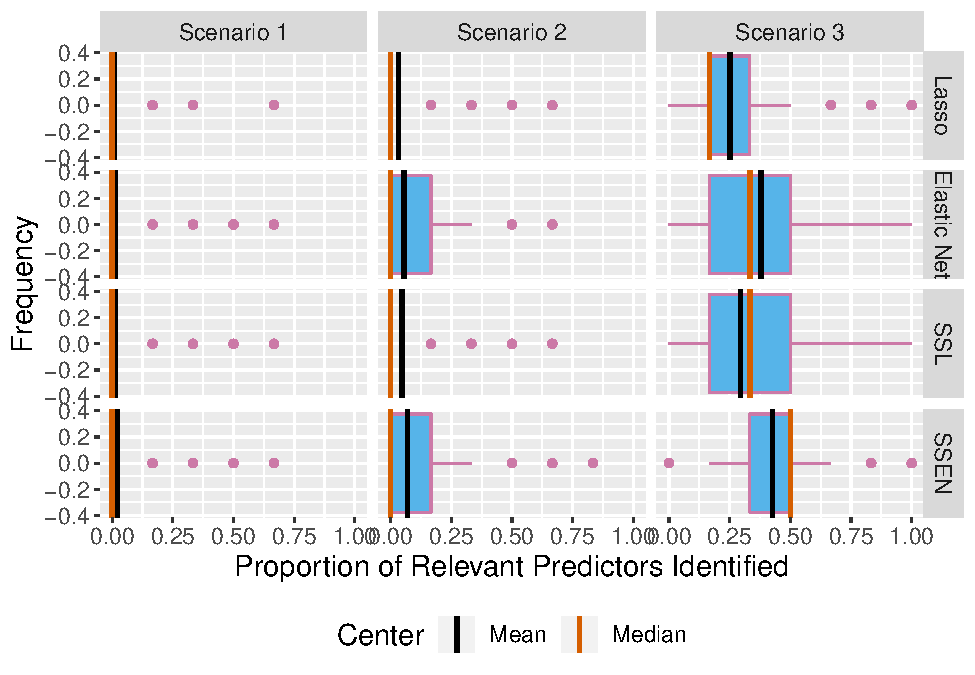
\includegraphics{simulation_results_files/figure-latex/unnamed-chunk-24-2.pdf}

\end{document}
